\documentclass[12pt, a4paper]{article}

\usepackage[top=2.5cm, bottom=2.5cm, left=2.5cm, right=2.5cm]{geometry}
\usepackage{graphicx}
\usepackage{amsmath, amssymb, amsfonts}
\usepackage{caption}
\usepackage{subcaption}
\usepackage{booktabs}
\usepackage{array}
\usepackage{float}
\usepackage{hyperref}
\usepackage{listings}
\usepackage{xcolor}
\usepackage{fancyhdr}
\usepackage{titlesec}
\usepackage{tocloft}
\usepackage{setspace}
\usepackage{cite}
\usepackage{url}
\usepackage{parskip}

\lstset{
  language=Python,
  basicstyle=\ttfamily\footnotesize,
  keywordstyle=\color{blue}\bfseries,
  commentstyle=\color{gray}\itshape,
  stringstyle=\color{red!70!black},
  numberstyle=\tiny\color{gray},
  numbers=left,
  stepnumber=1,
  numbersep=8pt,
  breaklines=true,
  breakatwhitespace=false,
  frame=single,
  rulecolor=\color{black!30},
  backgroundcolor=\color{gray!5},
  captionpos=b,
  tabsize=4,
  showstringspaces=false,
  xleftmargin=15pt,
  xrightmargin=5pt
}

\pagestyle{fancy}
\fancyhf{}
\fancyhead[L]{\small EE 325 Digital Signal Processing}
\fancyhead[R]{\small Laboratory Report 02}
\fancyfoot[C]{\thepage}
\renewcommand{\headrulewidth}{0.4pt}
\setlength{\headheight}{14pt}

\begin{document}
\pagenumbering{gobble}
\begin{titlepage}
  \begin{center}
    \vspace*{1cm}
    {\large \textbf{UNIVERSITY OF PERADENIYA}} \\[0.3cm]
    {\large Faculty of Engineering} \\[0.3cm]
    {\large Department of Electrical and Electronic Engineering} \\[2cm]

    \rule{\linewidth}{0.5mm} \\[0.4cm]
    {\LARGE \textbf{EE 325: Digital Signal Processing}} \\[0.3cm]
    {\Large \textbf{Laboratory Report 02}} \\[0.3cm]
    {\Large Digital Filter Design and Comparative Analysis} \\[0.2cm]
    \rule{\linewidth}{0.5mm} \\[2cm]

    \begin{tabular}{ll}
      \textbf{Student Name:}    & Dineth Perera \\[0.2cm]
      \textbf{Registration No:} & E/21/291 \\[0.2cm]
      \textbf{Degree Program:}  & B.Sc. Engineering (Electrical \& Electronic) \\[0.2cm]
      \textbf{Academic Year:}   & 2024/2025 \\[0.2cm]
      \textbf{Date Submitted:}  & \today \\[0.2cm]
    \end{tabular}

    \vfill
    {\small Department of Electrical and Electronic Engineering \\
    University of Peradeniya, Peradeniya 20400, Sri Lanka}
  \end{center}
\end{titlepage}

\clearpage
\pagenumbering{arabic}
\tableofcontents
\newpage

\section{Introduction}
Digital filter design is central to signal conditioning because a practical processing chain must retain desired spectral content while attenuating unwanted components. In discrete-time systems, this design problem is shaped by several coupled constraints: passband fidelity, stopband attenuation, transition width, stability, implementation cost, and phase linearity \cite{oppenheim2010, proakis2007, mitra2011}. This laboratory compares three classical IIR low-pass filters and five window-based FIR low-pass filters under a single specification set derived from the student number E/21/291, then evaluates their responses for both noise and chirp inputs.

For this registration number, the required digits are $a=2$, $b=9$, $c=1$, and the digit sum is $2+9+1=12$, which gives $d=1+2=3$. Therefore,
\begin{equation}
\omega_p = 100 + \sqrt{1.1(2) + 11(9) + 101(1)} = 100 + \sqrt{202.2} \approx 114.22\ \text{rad/s},
\end{equation}
\begin{equation}
\omega_s = \omega_p \left(1 + \sqrt{\frac{3}{10}}\right) \approx 176.78\ \text{rad/s},
\end{equation}
with
\begin{equation}
\delta_s = 0.1, \qquad \delta_p = 0.9, \qquad \delta_t = 0.1.
\end{equation}
The filters designed in this report are Butterworth, Chebyshev Type I, Chebyshev Type II, and FIR filters using boxcar, Bartlett, Hann, Hamming, and Blackman windows. These are interpreted using the systems perspective of \cite{oppenheim2010, proakis2007, mitra2011, oppenheim1997}.

\section{Task 1: Filter Order Comparison}
The first task was to derive the orders required to satisfy the specifications. For the IIR designs, the digital specification is interpreted through the bilinear transform, so the passband and stopband edges are prewarped as
\begin{equation}
\Omega_p = 2F_s \tan\left(\frac{\omega_p}{2F_s}\right) = 114.3440\ \text{rad/s},
\end{equation}
\begin{equation}
\Omega_s = 2F_s \tan\left(\frac{\omega_s}{2F_s}\right) = 177.2422\ \text{rad/s},
\end{equation}
with $F_s = 1000$ Sa/s. The passband and stopband ripple parameters are
\begin{equation}
\epsilon_p = \sqrt{\frac{1}{\delta_p^2} - 1} = \sqrt{\frac{1}{0.9^2} - 1} \approx 0.4843,
\end{equation}
\begin{equation}
\epsilon_s = \sqrt{\frac{1}{\delta_s^2} - 1} = \sqrt{\frac{1}{0.1^2} - 1} \approx 9.9499,
\end{equation}
and the warped edge ratio is
\begin{equation}
\frac{\Omega_s}{\Omega_p} = 1.5501.
\end{equation}

For the Butterworth design,
\begin{equation}
N_{\mathrm{B}} \ge \frac{\log(\epsilon_s / \epsilon_p)}{\log(\Omega_s / \Omega_p)} = 6.8960,
\end{equation}
so the minimum order is $N_{\mathrm{B}} = 7$. For Chebyshev Type I and Type II,
\begin{equation}
N_{\mathrm{C}} \ge \frac{\cosh^{-1}(\epsilon_s / \epsilon_p)}{\cosh^{-1}(\Omega_s / \Omega_p)} = 3.6932,
\end{equation}
so both designs require order 4. These manual results were verified against \texttt{scipy.signal.buttord}, \texttt{cheb1ord}, and \texttt{cheb2ord}, and the software returned the same orders.

For the FIR designs, the transition bandwidth is
\begin{equation}
\Delta \omega = \omega_s - \omega_p = 62.5607\ \text{rad/s},
\end{equation}
which gives the normalized digital transition width
\begin{equation}
\Delta \omega_{\mathrm{norm}} = \frac{\Delta \omega}{F_s} = 0.0625607\ \text{rad/sample}.
\end{equation}
Applying the requested window-order formulas gives
\begin{equation}
N_{\mathrm{box}} = \left\lceil \frac{4\pi}{\Delta \omega_{\mathrm{norm}}} \right\rceil - 1 = 200,
\end{equation}
\begin{equation}
N_{\mathrm{bart}} = N_{\mathrm{hann}} = N_{\mathrm{hamm}} = \left\lceil \frac{8\pi}{\Delta \omega_{\mathrm{norm}}} \right\rceil - 1 = 401,
\end{equation}
\begin{equation}
N_{\mathrm{black}} = \left\lceil \frac{12\pi}{\Delta \omega_{\mathrm{norm}}} \right\rceil - 1 = 602.
\end{equation}
To keep the FIR filters in symmetric Type-I form, the odd order 401 was adjusted to the nearest even order 402 so that the number of taps $N+1$ is odd and the coefficients remain exactly symmetric \cite{mitra2011, harris1978}.

The resulting order comparison is summarized in Table~\ref{tab:orders}.
\begin{table}[H]
  \centering
  \caption{Computed filter orders for E/21/291.}
  \label{tab:orders}
  \begin{tabular}{lcc}
    \toprule
    Filter Type & Order $N$ & Type \\
    \midrule
    Butterworth & 7 & IIR \\
    Chebyshev Type I & 4 & IIR \\
    Chebyshev Type II & 4 & IIR \\
    Boxcar (Rectangular) & 200 & FIR \\
    Bartlett & 402 & FIR \\
    Hann & 402 & FIR \\
    Hamming & 402 & FIR \\
    Blackman & 602 & FIR \\
    \bottomrule
  \end{tabular}
\end{table}

Table~\ref{tab:orders} confirms the expected trend: Chebyshev filters achieve the specifications at lower order than the Butterworth design because they permit controlled ripple, while the FIR window methods need much higher orders because they trade recursive efficiency for linear-phase behavior and direct convolution structure \cite{rabiner1975, parks1987, harris1978}.

\section{Task 2: Filter Transfer Functions}
The verified implementation uses the bilinear transform
\begin{equation}
s \mapsto \frac{2F_s(z-1)}{z+1}
\end{equation}
to map the analog low-pass IIR prototypes into stable digital filters \cite{oppenheim2010, antoniou2018, rabiner1975}. For each IIR design, the transfer function is represented in second-order-section form,
\begin{equation}
H(z) = \prod_{m=1}^{M} \frac{b_{0,m} + b_{1,m}z^{-1} + b_{2,m}z^{-2}}{1 + a_{1,m}z^{-1} + a_{2,m}z^{-2}}.
\end{equation}

The Butterworth section coefficients are listed in Table~\ref{tab:buttersos}, the Chebyshev Type I coefficients in Table~\ref{tab:cheby1sos}, and the Chebyshev Type II coefficients in Table~\ref{tab:cheby2sos}. These tables define the digital transfer functions explicitly without printing unwieldy high-order polynomials.
\begin{table}[H]
  \centering
  \footnotesize
  \caption{Butterworth SOS coefficients.}
  \label{tab:buttersos}
  \begin{tabular}{cccccc}
    \toprule
    Sec. & $b_0$ & $b_1$ & $b_2$ & $a_1$ & $a_2$ \\
    \midrule
    1 & $3.10\times10^{-9}$ & $6.27\times10^{-9}$ & $3.17\times10^{-9}$ & $-0.8807$ & $0.0000$ \\
    2 & $1.0000$ & $2.0050$ & $1.0051$ & $-1.7813$ & $0.7956$ \\
    3 & $1.0000$ & $1.9857$ & $0.9859$ & $-1.8391$ & $0.8540$ \\
    4 & $1.0000$ & $0.9886$ & $0.0000$ & $-1.9297$ & $0.9453$ \\
    \bottomrule
  \end{tabular}
\end{table}

\begin{table}[H]
  \centering
  \footnotesize
  \caption{Chebyshev Type I SOS coefficients.}
  \label{tab:cheby1sos}
  \begin{tabular}{cccccc}
    \toprule
    Sec. & $b_0$ & $b_1$ & $b_2$ & $a_1$ & $a_2$ \\
    \midrule
    1 & $2.60\times10^{-6}$ & $5.20\times10^{-6}$ & $2.60\times10^{-6}$ & $-1.9200$ & $0.9236$ \\
    2 & $1.0000$ & $2.0000$ & $1.0000$ & $-1.9549$ & $0.9677$ \\
    \bottomrule
  \end{tabular}
\end{table}

\begin{table}[H]
  \centering
  \footnotesize
  \caption{Chebyshev Type II SOS coefficients.}
  \label{tab:cheby2sos}
  \begin{tabular}{cccccc}
    \toprule
    Sec. & $b_0$ & $b_1$ & $b_2$ & $a_1$ & $a_2$ \\
    \midrule
    1 & $0.08740$ & $-0.15885$ & $0.08740$ & $-1.7045$ & $0.7339$ \\
    2 & $1.0000$ & $-1.9675$ & $1.0000$ & $-1.9161$ & $0.9338$ \\
    \bottomrule
  \end{tabular}
\end{table}

For the FIR window designs, the transfer functions are of the polynomial form
\begin{equation}
H_{\mathrm{FIR}}(z) = \sum_{k=0}^{N} b[k] z^{-k},
\end{equation}
with symmetric coefficients $b[k] = b[N-k]$, which guarantees linear phase. The polynomial degrees are 200 for the boxcar filter, 402 for the Bartlett, Hann, and Hamming filters, and 602 for the Blackman filter. Because these coefficient vectors are long, the full numerical arrays are placed in the appendix code listings rather than expanded in the main text \cite{proakis2007, mitra2011, harris1978}.

\section{Task 3: Pole-Zero Plots, Impulse Response, Frequency Response, and Group Delay}
Task 3 required a complete response study for each of the eight filters. The passband edge is
\begin{equation}
f_p = \frac{\omega_p}{2\pi} = 18.1786\ \text{Hz},
\end{equation}
the stopband edge is
\begin{equation}
f_s = \frac{\omega_s}{2\pi} = 28.1355\ \text{Hz},
\end{equation}
and the FIR midpoint cutoff used in the design is
\begin{equation}
f_c = \frac{\omega_p + \omega_s}{4\pi} = 23.1571\ \text{Hz}.
\end{equation}

\subsection{Butterworth Filter}
Figures~\ref{fig:butter_pz}--\ref{fig:butter_gd} summarize the Butterworth filter responses. The pole-zero plot confirms stability because all poles lie strictly inside the unit circle. The gain response meets the minimum passband gain requirement with measured $\min |H| = 0.9072$ and the stopband requirement with measured $\max |H| = 0.0941$ beyond the stopband edge.
\begin{figure}[H]
  \centering
  \begin{subfigure}{0.48\textwidth}
    \centering
    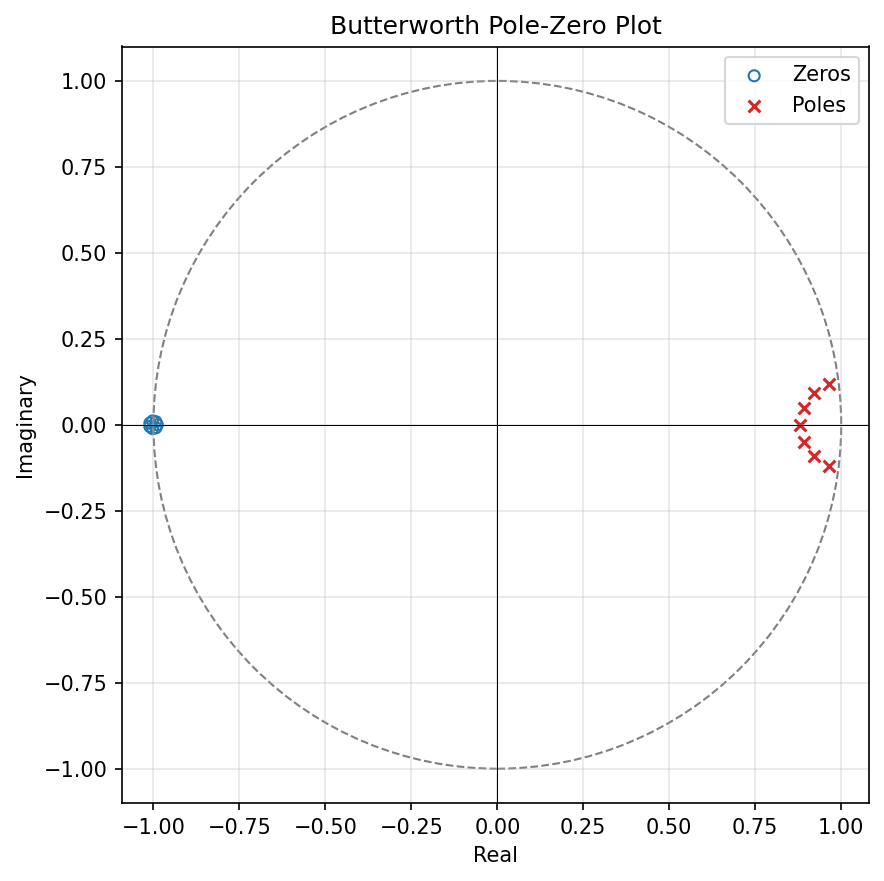
\includegraphics[width=\textwidth]{lab02_fig02_butter_pz.png}
    \caption{Pole-zero plot}
    \label{fig:butter_pz}
  \end{subfigure}
  \hfill
  \begin{subfigure}{0.48\textwidth}
    \centering
    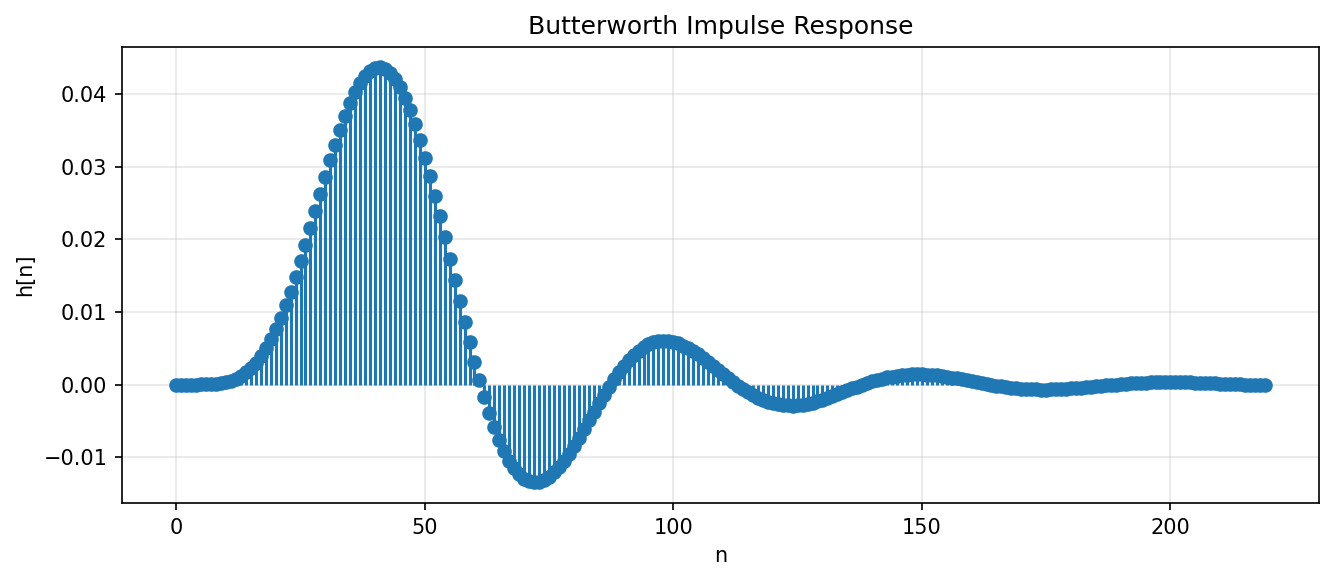
\includegraphics[width=\textwidth]{lab02_fig03_butter_impulse.png}
    \caption{Impulse response}
    \label{fig:butter_imp}
  \end{subfigure}
  \caption{Butterworth pole-zero plot and impulse response.}
\end{figure}

\begin{figure}[H]
  \centering
  \begin{subfigure}{0.32\textwidth}
    \centering
    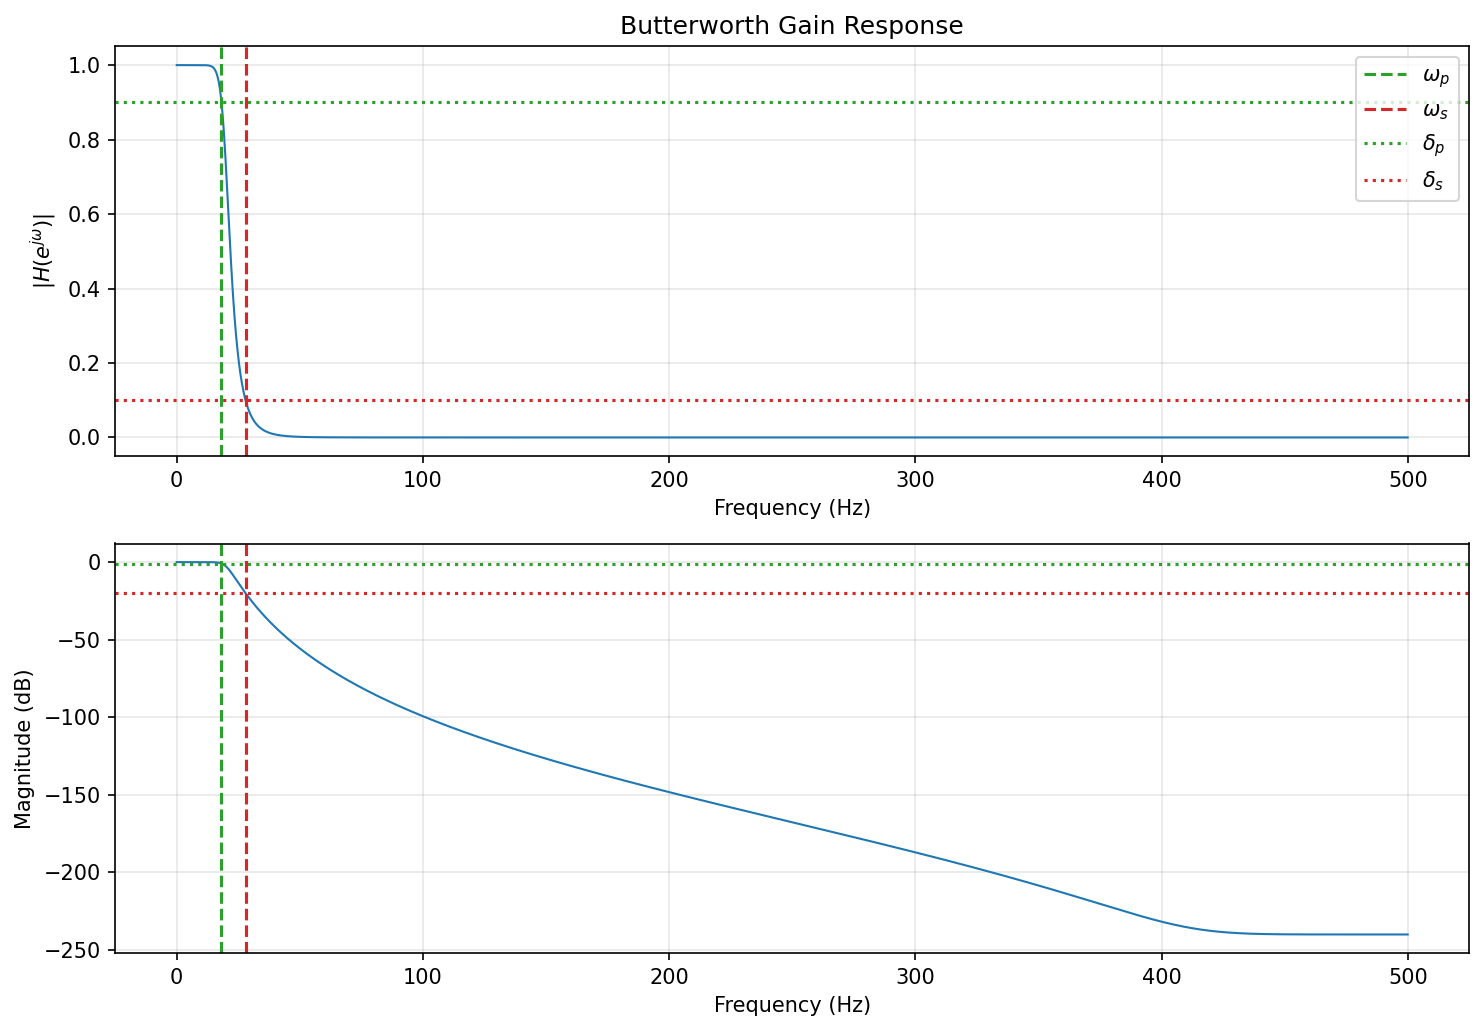
\includegraphics[width=\textwidth]{lab02_fig04_butter_gain.png}
    \caption{Gain response}
    \label{fig:butter_gain}
  \end{subfigure}
  \hfill
  \begin{subfigure}{0.32\textwidth}
    \centering
    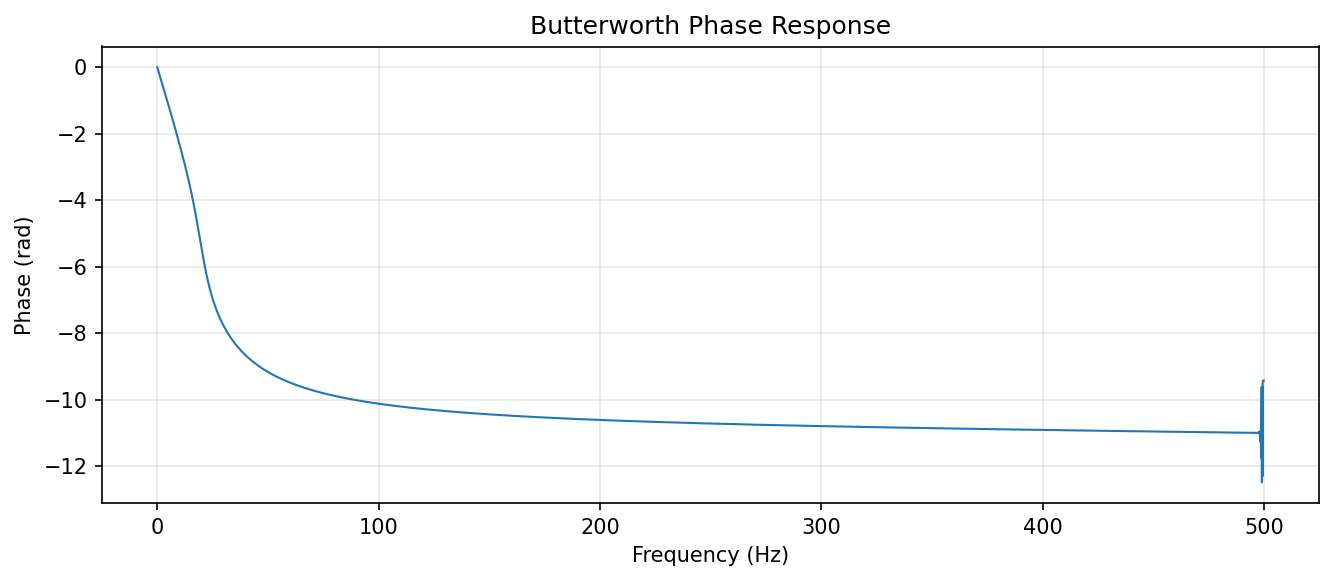
\includegraphics[width=\textwidth]{lab02_fig05_butter_phase.png}
    \caption{Phase response}
    \label{fig:butter_phase}
  \end{subfigure}
  \hfill
  \begin{subfigure}{0.32\textwidth}
    \centering
    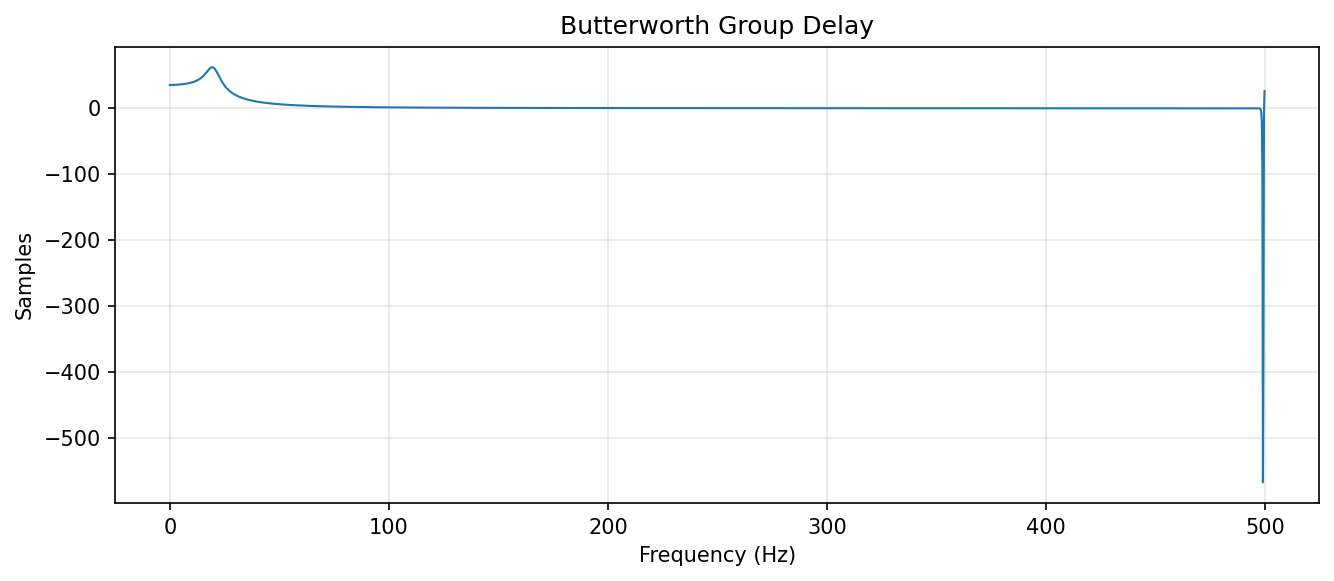
\includegraphics[width=\textwidth]{lab02_fig06_butter_gd.png}
    \caption{Group delay}
    \label{fig:butter_gd}
  \end{subfigure}
  \caption{Butterworth gain, phase, and group-delay characteristics.}
\end{figure}

The Butterworth passband is maximally flat, the roll-off is monotonic, and the impulse response decays gradually, confirming the infinite-duration nature of the IIR realization. The phase and group delay plots are nonlinear, so time-domain waveforms will experience frequency-dependent delay.

\subsection{Chebyshev Type I Filter}
Figures~\ref{fig:cheby1_pz}--\ref{fig:cheby1_gd} summarize the Chebyshev Type I design. The measured passband minimum is exactly 0.9000 and the stopband maximum is 0.0728, so the filter satisfies both constraints at a lower order than the Butterworth design.
\begin{figure}[H]
  \centering
  \begin{subfigure}{0.48\textwidth}
    \centering
    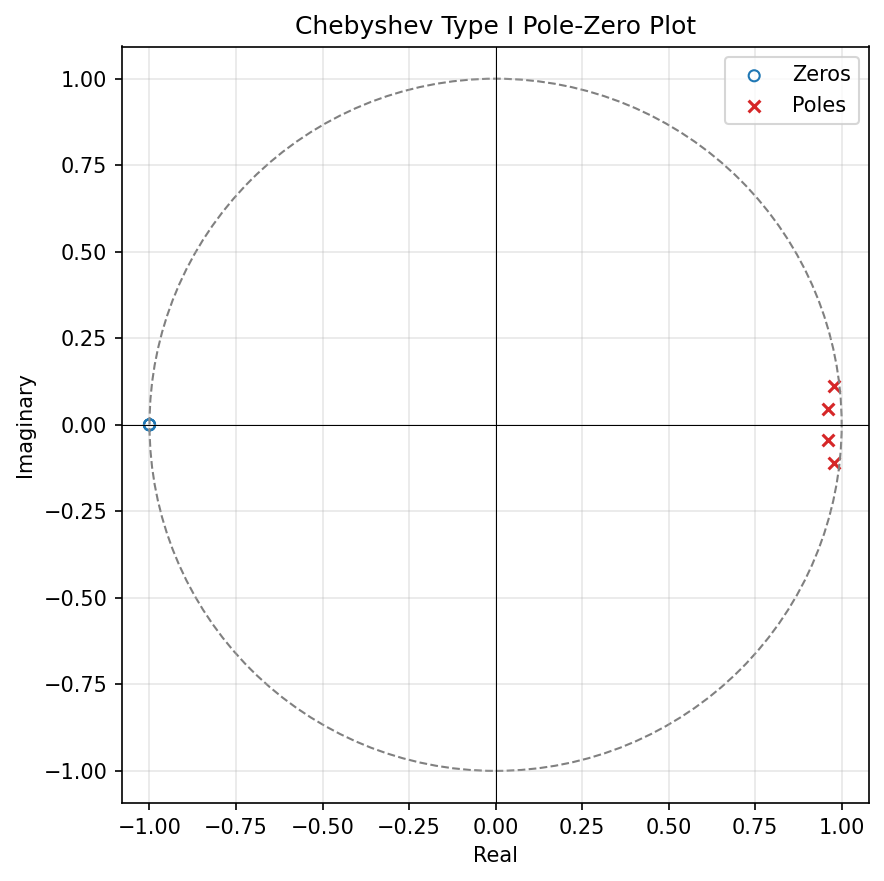
\includegraphics[width=\textwidth]{lab02_fig02_cheby1_pz.png}
    \caption{Pole-zero plot}
    \label{fig:cheby1_pz}
  \end{subfigure}
  \hfill
  \begin{subfigure}{0.48\textwidth}
    \centering
    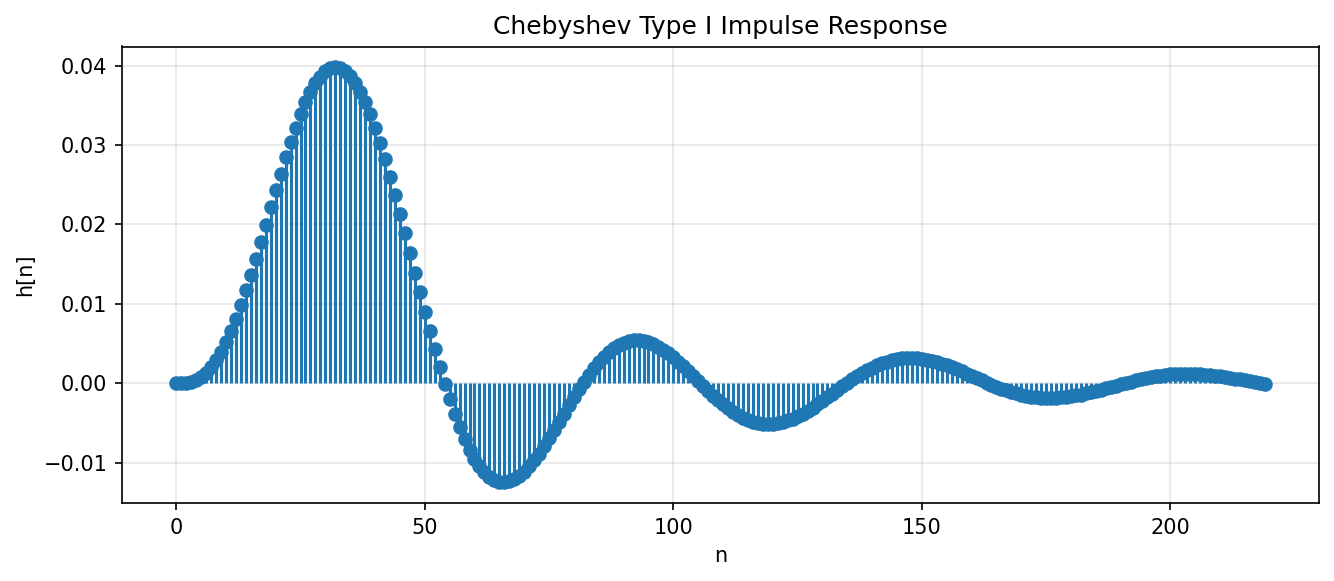
\includegraphics[width=\textwidth]{lab02_fig03_cheby1_impulse.png}
    \caption{Impulse response}
    \label{fig:cheby1_imp}
  \end{subfigure}
  \caption{Chebyshev Type I pole-zero plot and impulse response.}
\end{figure}

\begin{figure}[H]
  \centering
  \begin{subfigure}{0.32\textwidth}
    \centering
    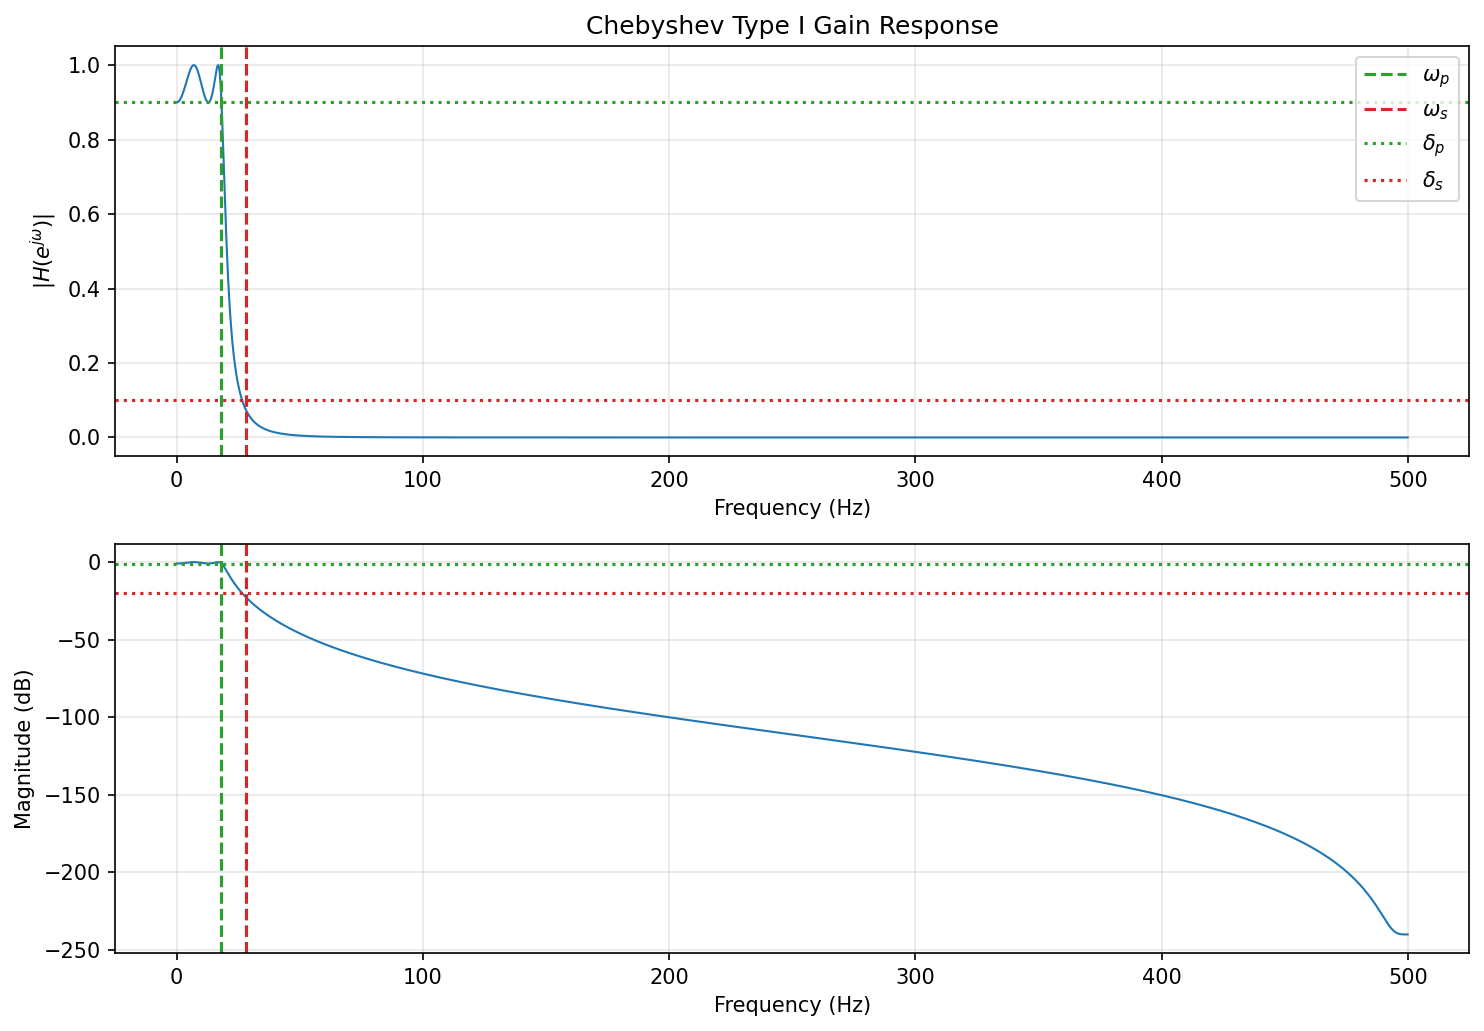
\includegraphics[width=\textwidth]{lab02_fig04_cheby1_gain.png}
    \caption{Gain response}
    \label{fig:cheby1_gain}
  \end{subfigure}
  \hfill
  \begin{subfigure}{0.32\textwidth}
    \centering
    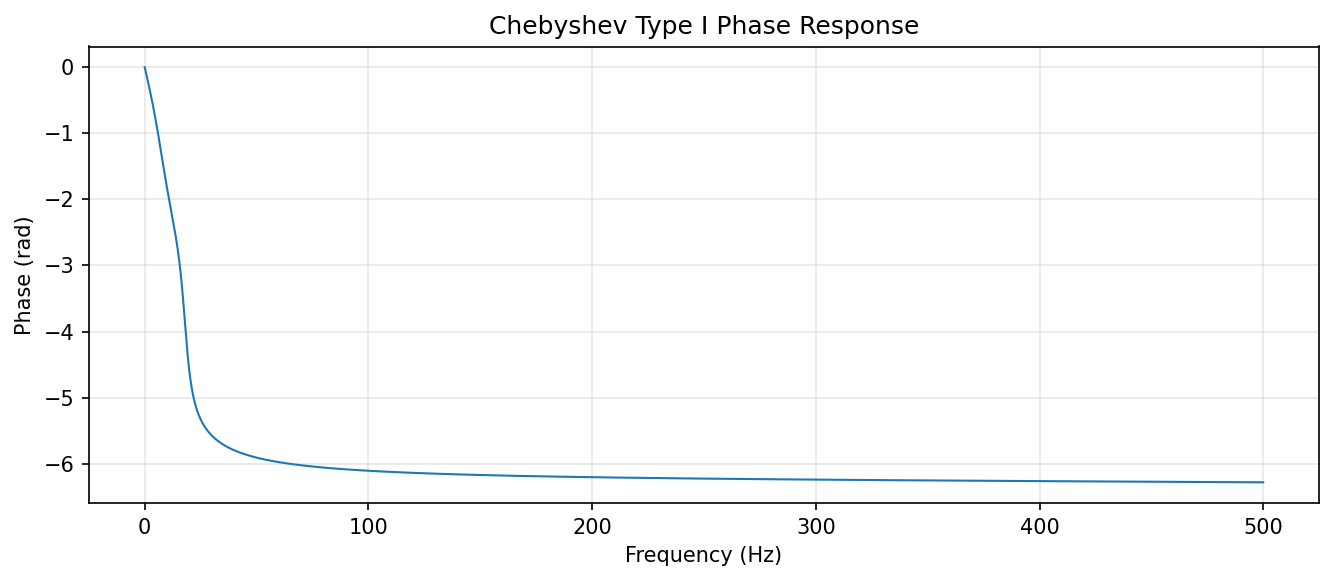
\includegraphics[width=\textwidth]{lab02_fig05_cheby1_phase.png}
    \caption{Phase response}
    \label{fig:cheby1_phase}
  \end{subfigure}
  \hfill
  \begin{subfigure}{0.32\textwidth}
    \centering
    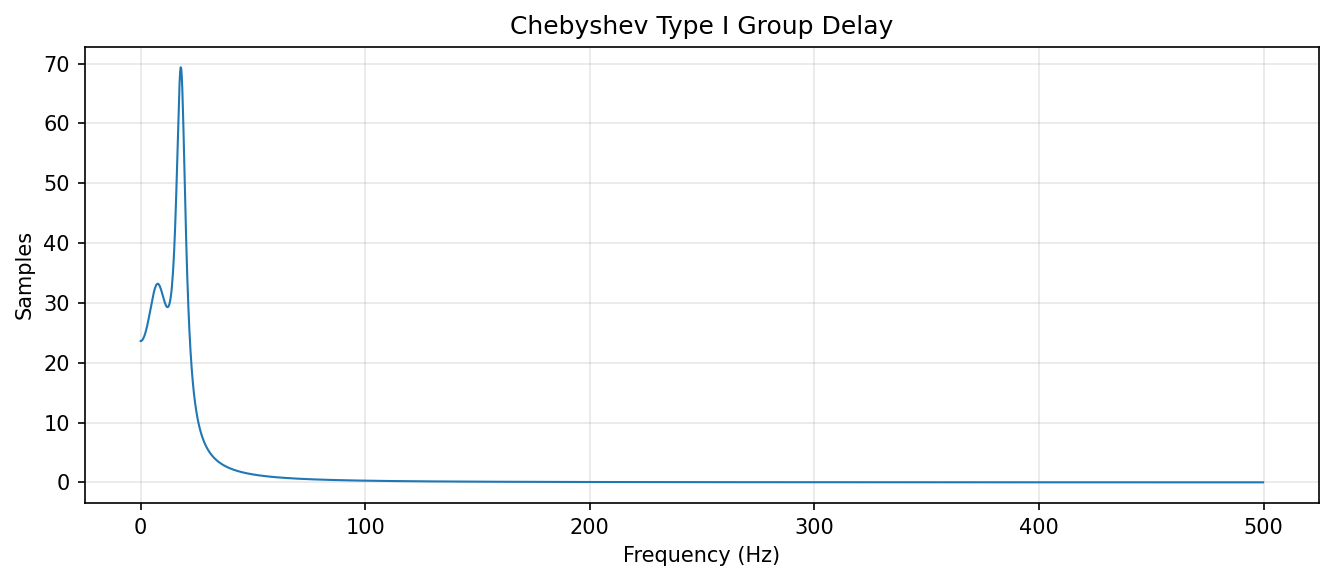
\includegraphics[width=\textwidth]{lab02_fig06_cheby1_gd.png}
    \caption{Group delay}
    \label{fig:cheby1_gd}
  \end{subfigure}
  \caption{Chebyshev Type I gain, phase, and group-delay characteristics.}
\end{figure}

The gain plot shows equiripple behavior in the passband and monotonic attenuation in the stopband, which is the defining trade-off of Chebyshev Type I filters. The phase is more nonlinear than the Butterworth case, but the reduced order makes the magnitude transition sharper for the same design constraints \cite{rabiner1975, antoniou2018}.

\subsection{Chebyshev Type II Filter}
Figures~\ref{fig:cheby2_pz}--\ref{fig:cheby2_gd} show the Chebyshev Type II responses. The design achieves $\min |H| = 0.9057$ in the passband and $\max |H| = 0.1000$ in the stopband, matching the stopband-limited specification exactly.
\begin{figure}[H]
  \centering
  \begin{subfigure}{0.48\textwidth}
    \centering
    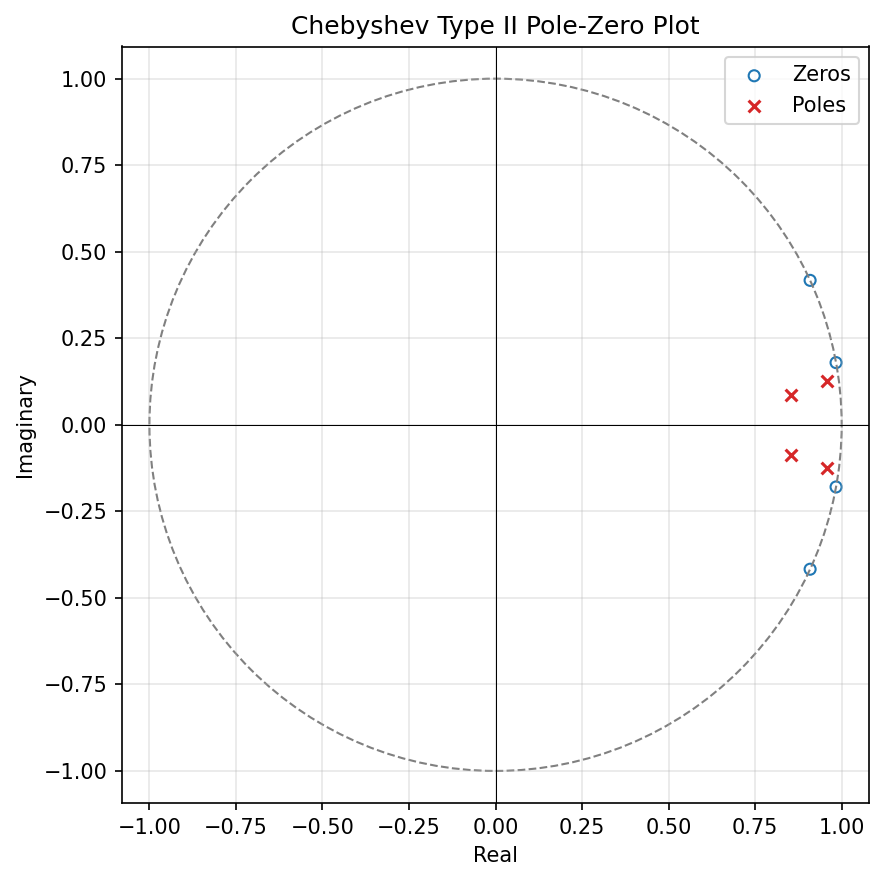
\includegraphics[width=\textwidth]{lab02_fig02_cheby2_pz.png}
    \caption{Pole-zero plot}
    \label{fig:cheby2_pz}
  \end{subfigure}
  \hfill
  \begin{subfigure}{0.48\textwidth}
    \centering
    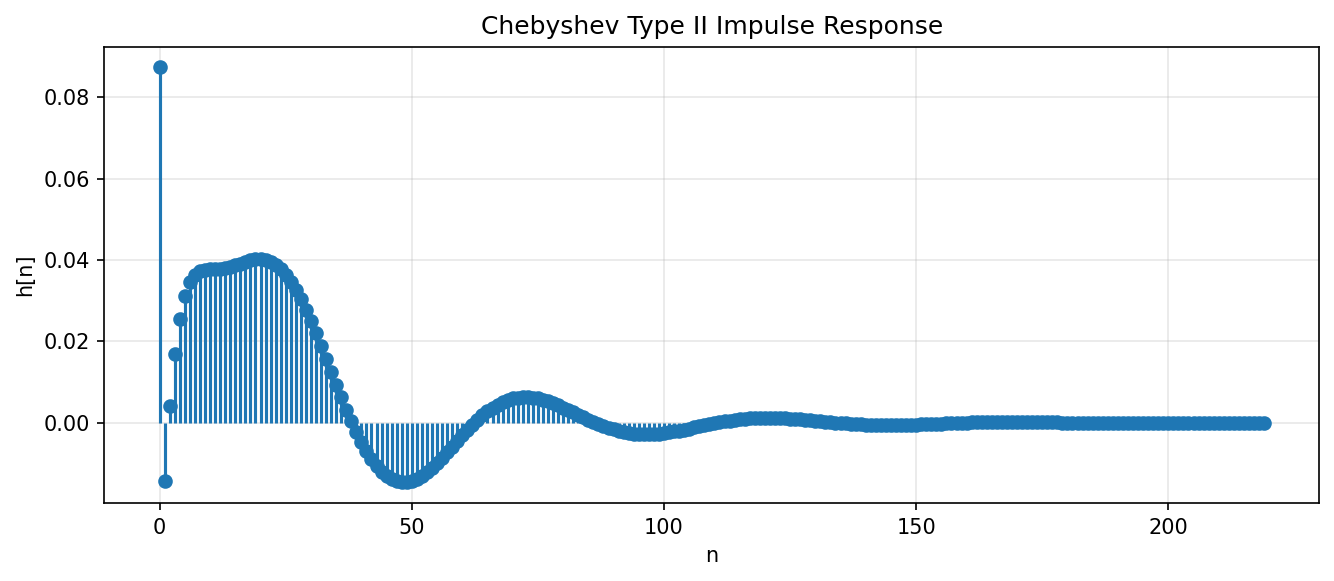
\includegraphics[width=\textwidth]{lab02_fig03_cheby2_impulse.png}
    \caption{Impulse response}
    \label{fig:cheby2_imp}
  \end{subfigure}
  \caption{Chebyshev Type II pole-zero plot and impulse response.}
\end{figure}

\begin{figure}[H]
  \centering
  \begin{subfigure}{0.32\textwidth}
    \centering
    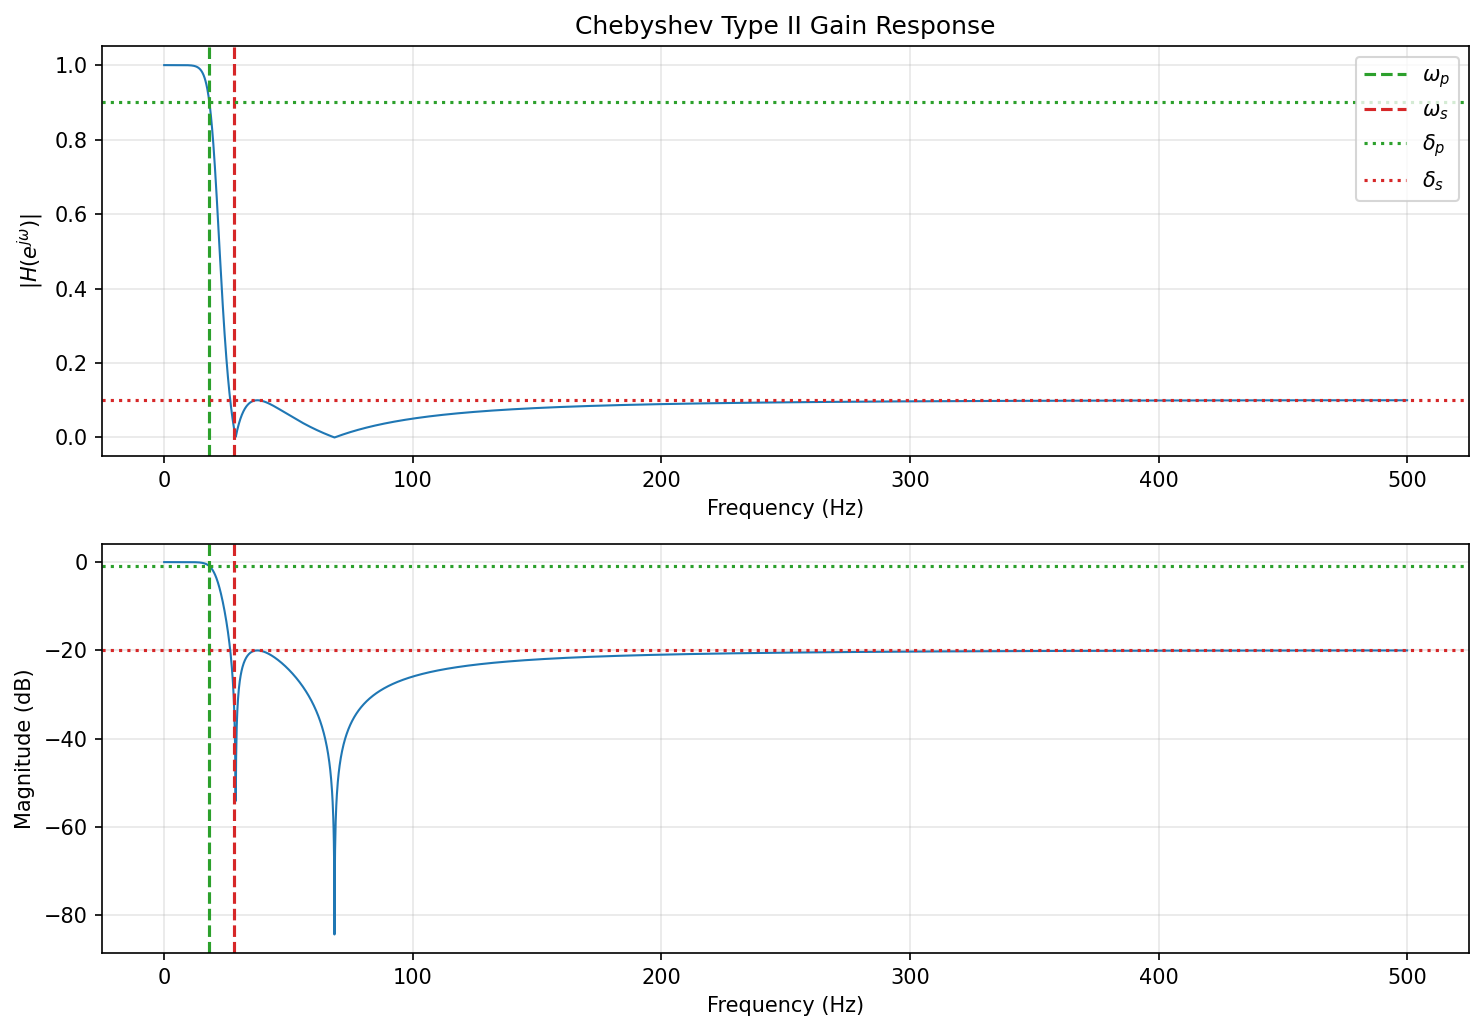
\includegraphics[width=\textwidth]{lab02_fig04_cheby2_gain.png}
    \caption{Gain response}
    \label{fig:cheby2_gain}
  \end{subfigure}
  \hfill
  \begin{subfigure}{0.32\textwidth}
    \centering
    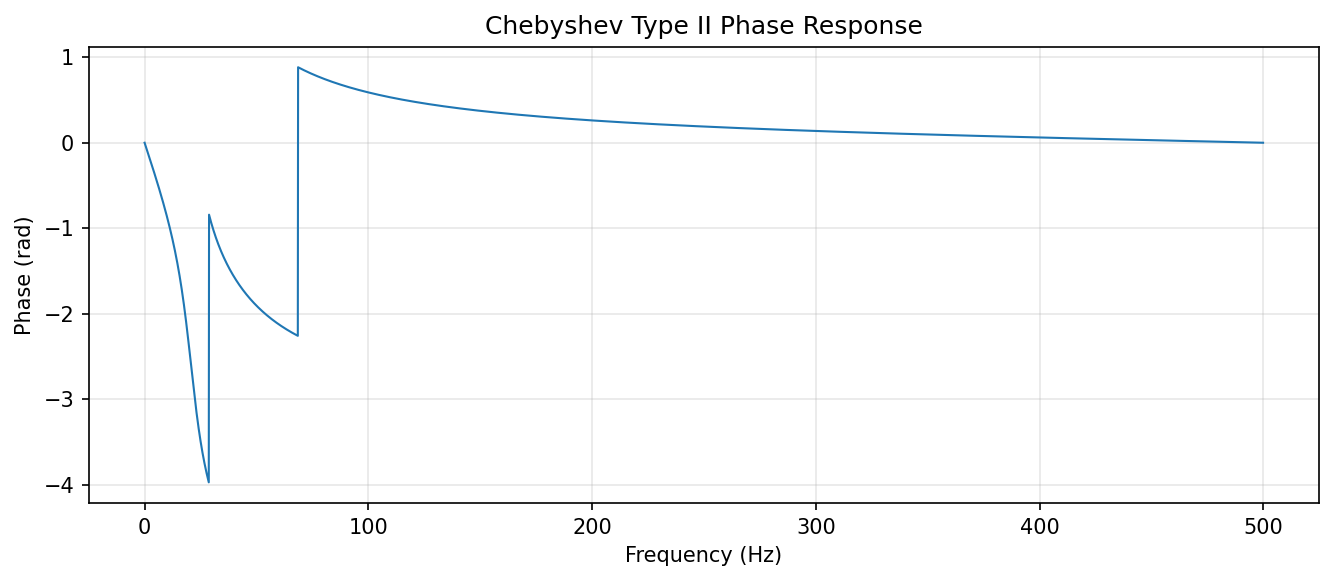
\includegraphics[width=\textwidth]{lab02_fig05_cheby2_phase.png}
    \caption{Phase response}
    \label{fig:cheby2_phase}
  \end{subfigure}
  \hfill
  \begin{subfigure}{0.32\textwidth}
    \centering
    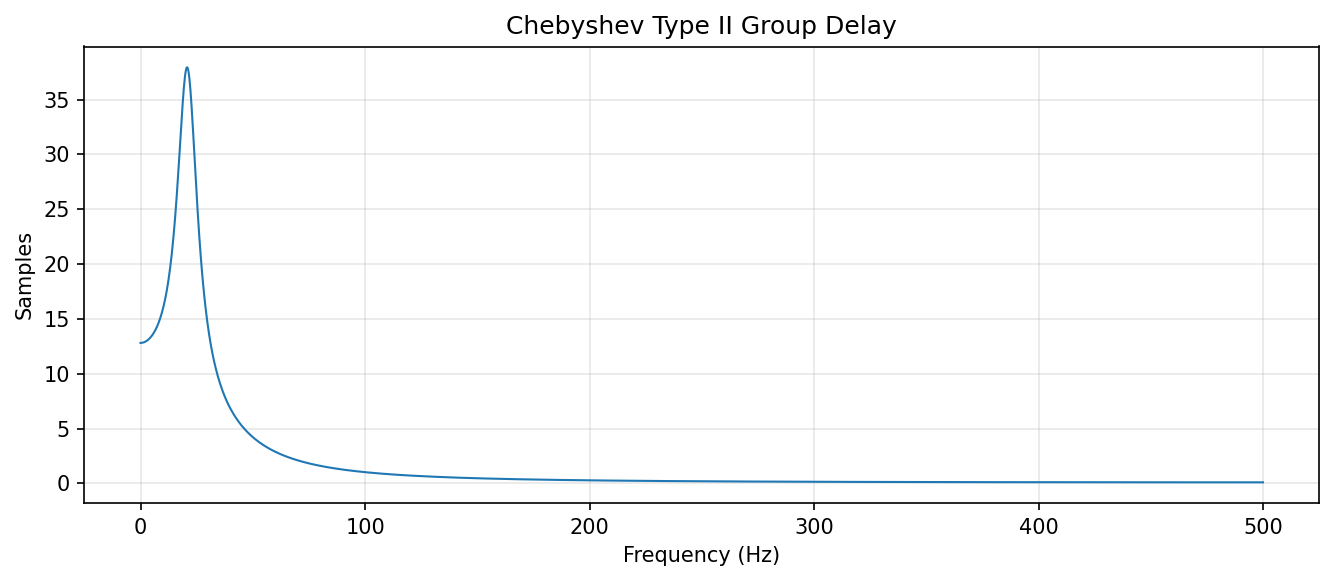
\includegraphics[width=\textwidth]{lab02_fig06_cheby2_gd.png}
    \caption{Group delay}
    \label{fig:cheby2_gd}
  \end{subfigure}
  \caption{Chebyshev Type II gain, phase, and group-delay characteristics.}
\end{figure}

The stopband ripple is evident in the gain response, and the pole-zero plot shows zeros close to the unit circle, which produce strong rejection notches. The passband remains monotonic, unlike the Type I case.

\subsection{Boxcar (Rectangular) Window FIR}
Figures~\ref{fig:box_pz}--\ref{fig:box_gd} show the boxcar FIR responses. The filter meets the numerical amplitude limits with $\min |H| = 0.9417$ and $\max |H| = 0.0932$, but its stopband sidelobes are visibly higher than those of the smoother windows.
\begin{figure}[H]
  \centering
  \begin{subfigure}{0.48\textwidth}
    \centering
    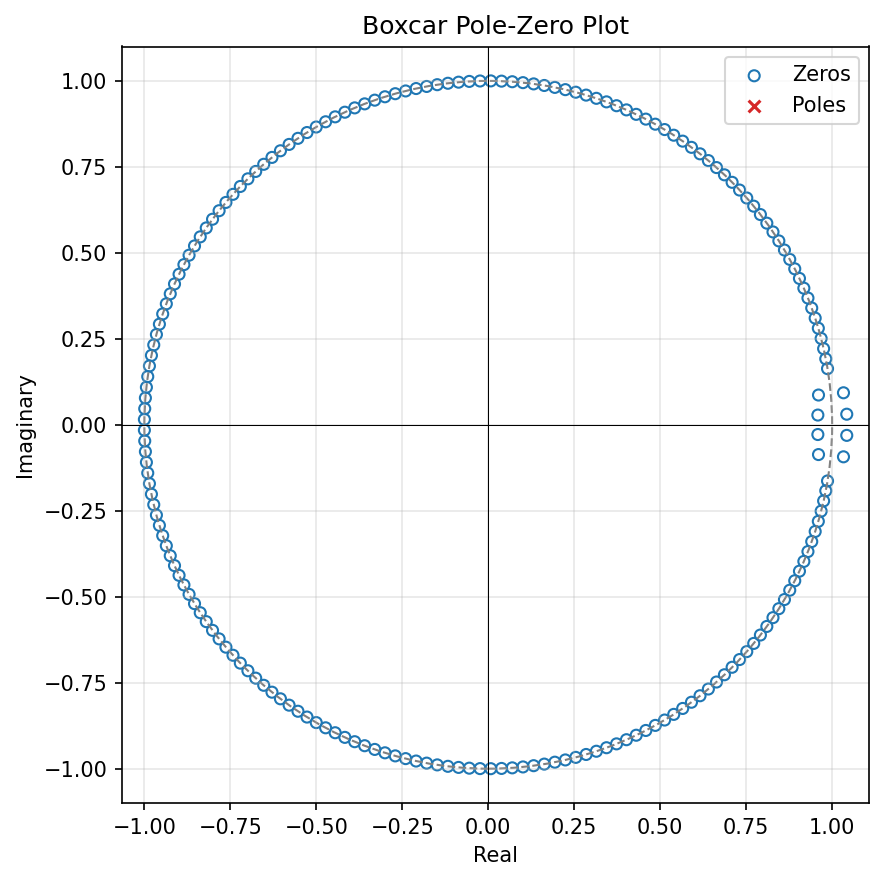
\includegraphics[width=\textwidth]{lab02_fig02_boxcar_pz.png}
    \caption{Pole-zero plot}
    \label{fig:box_pz}
  \end{subfigure}
  \hfill
  \begin{subfigure}{0.48\textwidth}
    \centering
    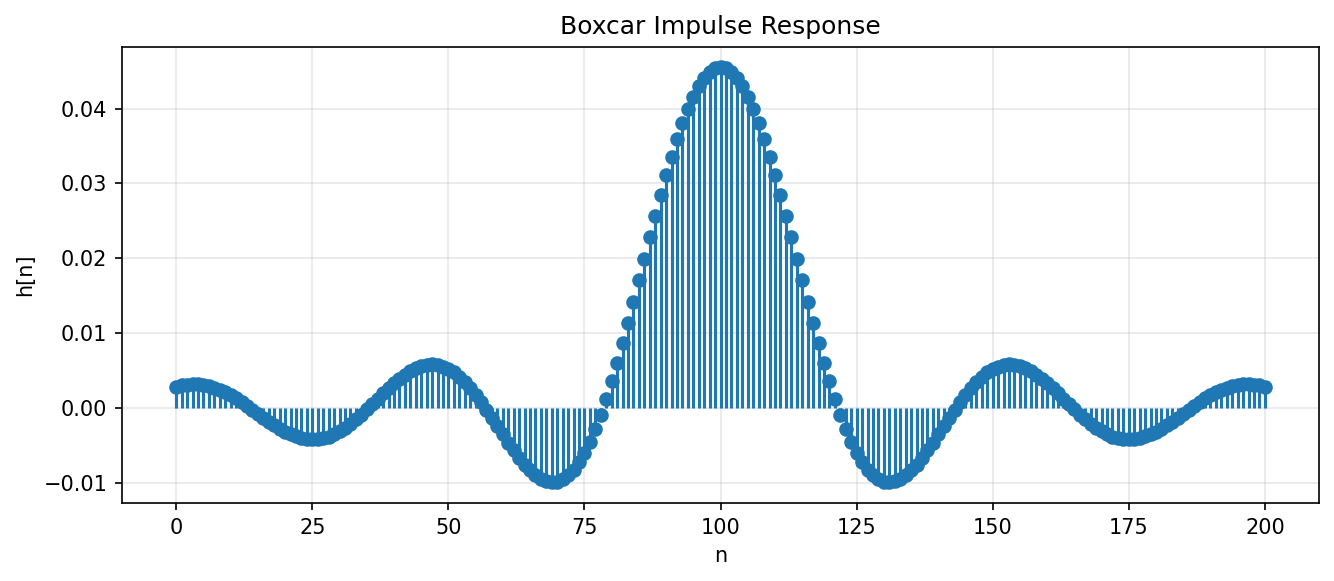
\includegraphics[width=\textwidth]{lab02_fig03_boxcar_impulse.png}
    \caption{Impulse response}
    \label{fig:box_imp}
  \end{subfigure}
  \caption{Boxcar FIR pole-zero plot and impulse response.}
\end{figure}

\begin{figure}[H]
  \centering
  \begin{subfigure}{0.32\textwidth}
    \centering
    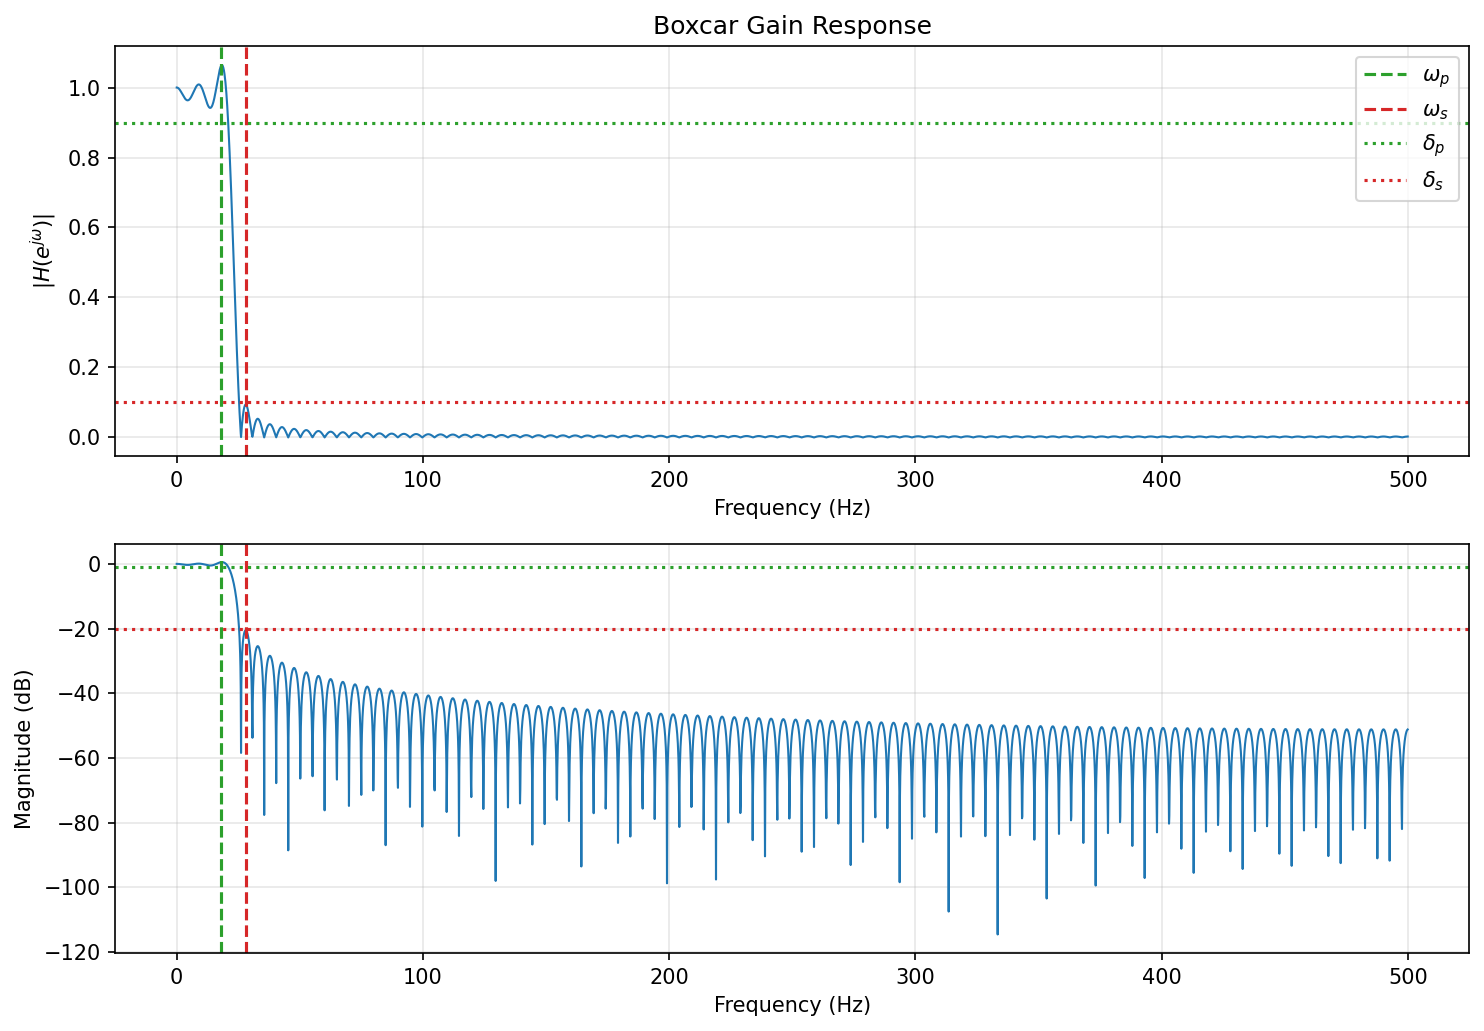
\includegraphics[width=\textwidth]{lab02_fig04_boxcar_gain.png}
    \caption{Gain response}
    \label{fig:box_gain}
  \end{subfigure}
  \hfill
  \begin{subfigure}{0.32\textwidth}
    \centering
    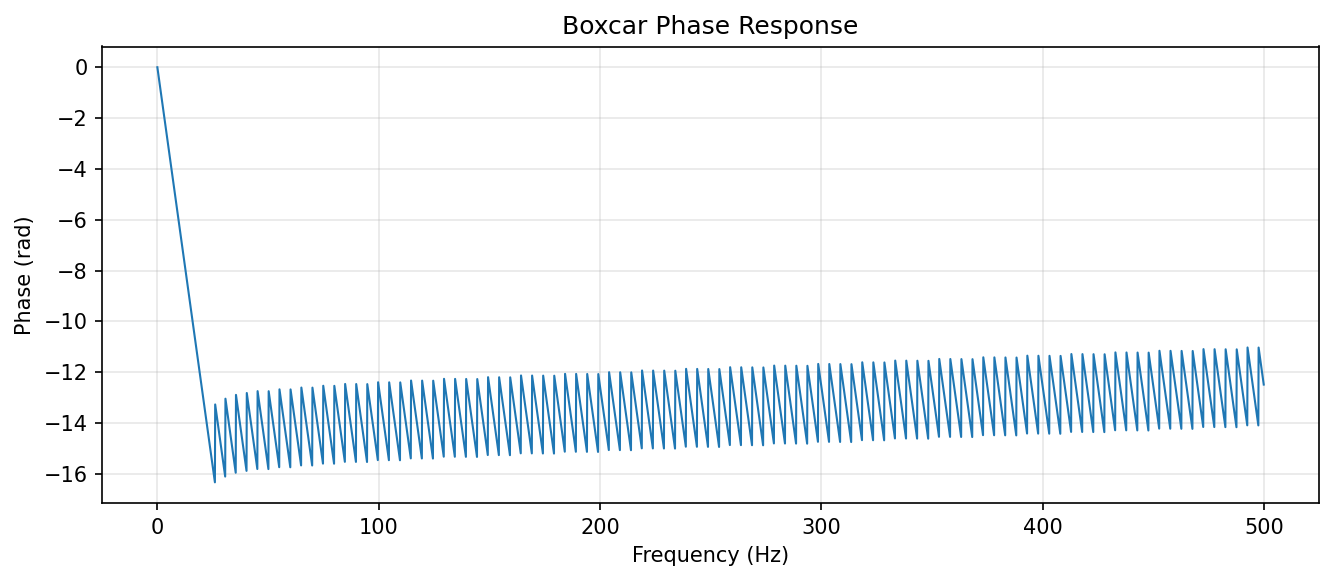
\includegraphics[width=\textwidth]{lab02_fig05_boxcar_phase.png}
    \caption{Phase response}
    \label{fig:box_phase}
  \end{subfigure}
  \hfill
  \begin{subfigure}{0.32\textwidth}
    \centering
    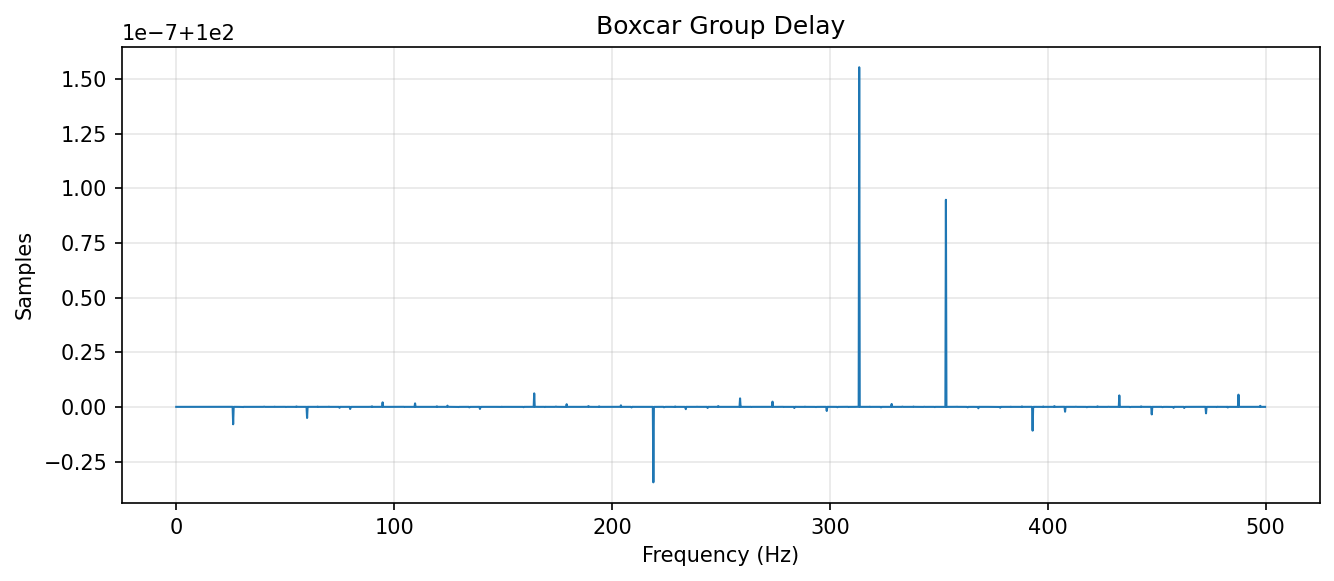
\includegraphics[width=\textwidth]{lab02_fig06_boxcar_gd.png}
    \caption{Group delay}
    \label{fig:box_gd}
  \end{subfigure}
  \caption{Boxcar FIR gain, phase, and group-delay characteristics.}
\end{figure}

The impulse response is finite and symmetric, so the phase is approximately linear and the group delay is nearly constant at $N/2$ samples. The price for the relatively low order is poorer stopband suppression.

\subsection{Bartlett (Triangular) Window FIR}
Figures~\ref{fig:bart_pz}--\ref{fig:bart_gd} summarize the Bartlett window design. The measured gains are $\min |H| = 0.9656$ and $\max |H| = 0.0446$, showing better stopband suppression than the boxcar filter at the cost of a much higher order.
\begin{figure}[H]
  \centering
  \begin{subfigure}{0.48\textwidth}
    \centering
    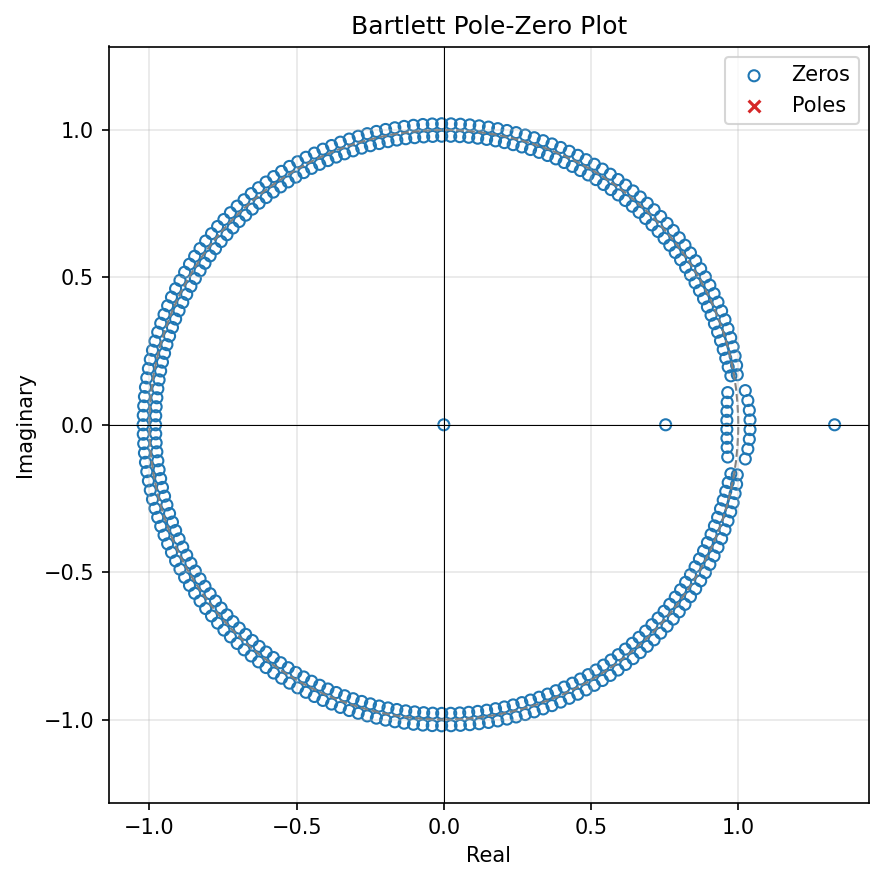
\includegraphics[width=\textwidth]{lab02_fig02_bartlett_pz.png}
    \caption{Pole-zero plot}
    \label{fig:bart_pz}
  \end{subfigure}
  \hfill
  \begin{subfigure}{0.48\textwidth}
    \centering
    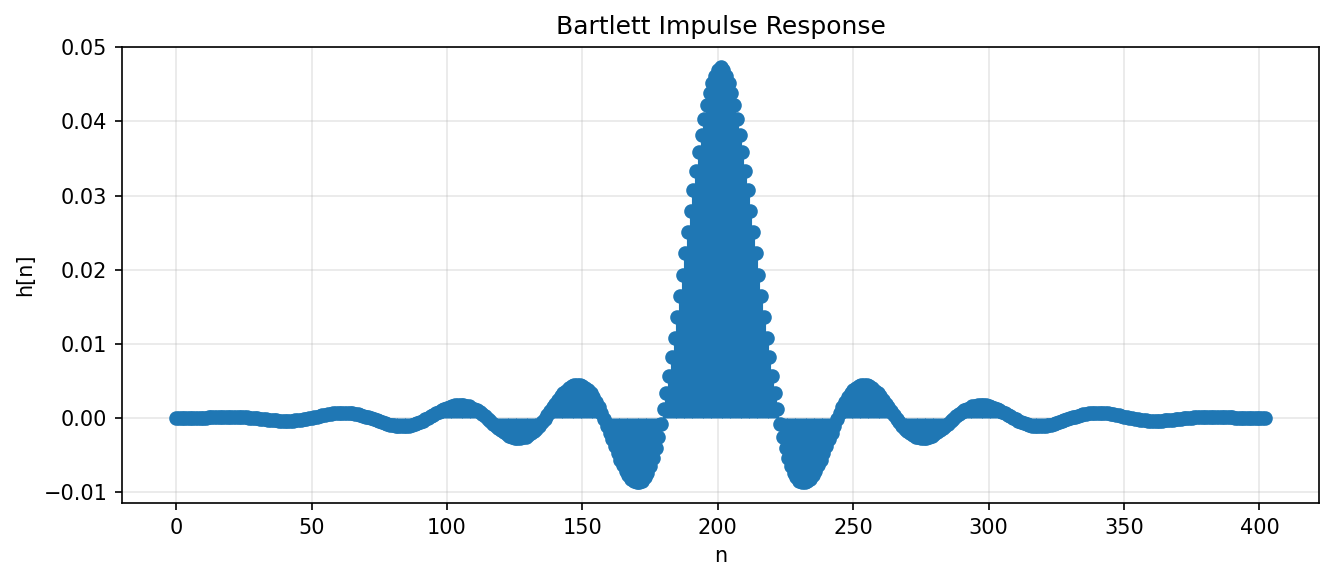
\includegraphics[width=\textwidth]{lab02_fig03_bartlett_impulse.png}
    \caption{Impulse response}
    \label{fig:bart_imp}
  \end{subfigure}
  \caption{Bartlett FIR pole-zero plot and impulse response.}
\end{figure}

\begin{figure}[H]
  \centering
  \begin{subfigure}{0.32\textwidth}
    \centering
    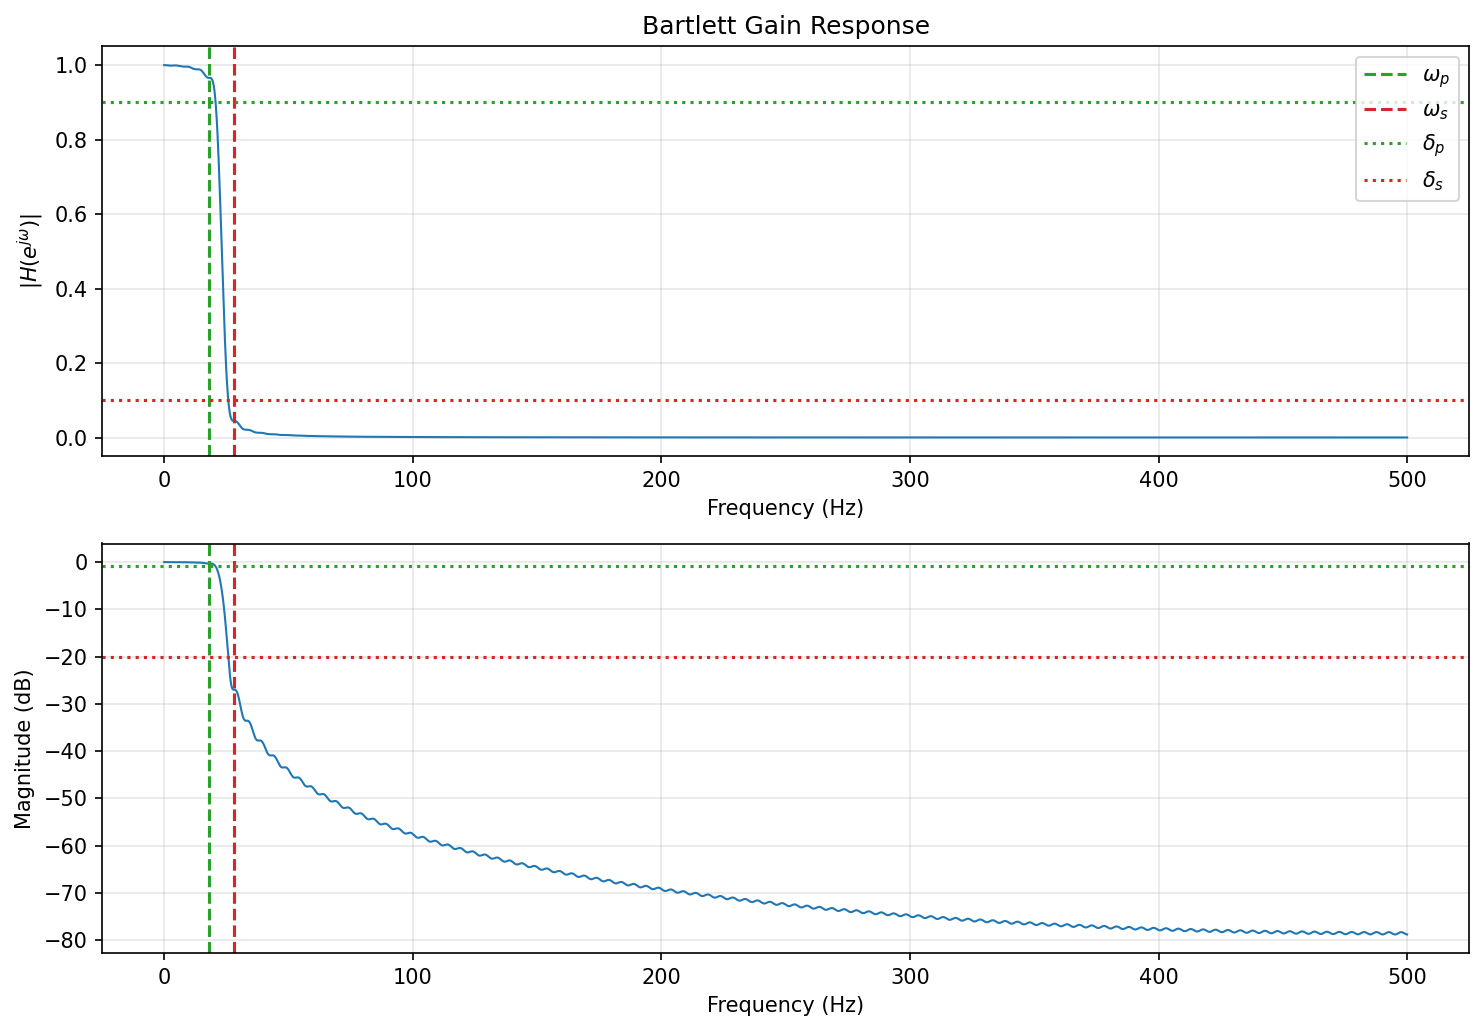
\includegraphics[width=\textwidth]{lab02_fig04_bartlett_gain.png}
    \caption{Gain response}
    \label{fig:bart_gain}
  \end{subfigure}
  \hfill
  \begin{subfigure}{0.32\textwidth}
    \centering
    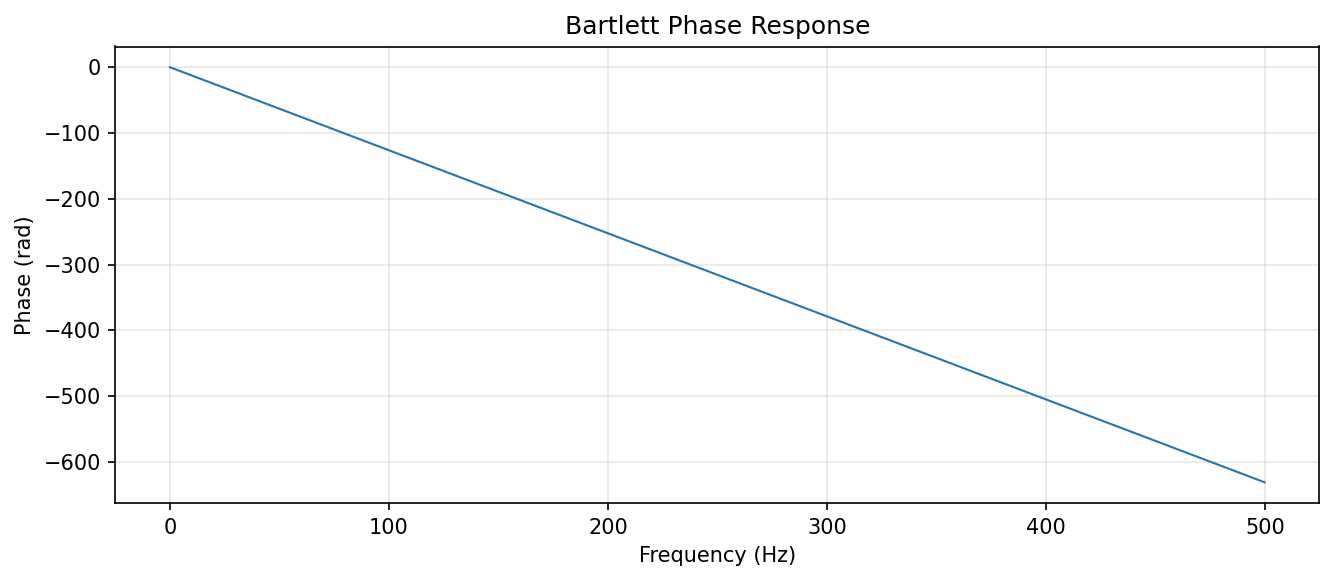
\includegraphics[width=\textwidth]{lab02_fig05_bartlett_phase.png}
    \caption{Phase response}
    \label{fig:bart_phase}
  \end{subfigure}
  \hfill
  \begin{subfigure}{0.32\textwidth}
    \centering
    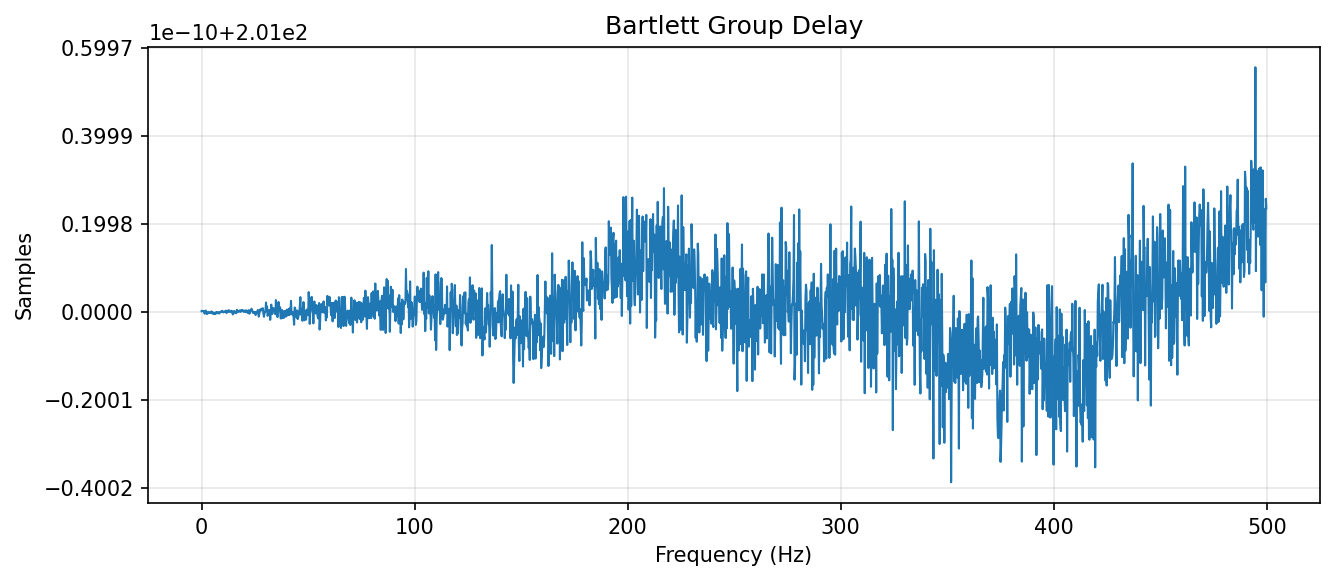
\includegraphics[width=\textwidth]{lab02_fig06_bartlett_gd.png}
    \caption{Group delay}
    \label{fig:bart_gd}
  \end{subfigure}
  \caption{Bartlett FIR gain, phase, and group-delay characteristics.}
\end{figure}

The sidelobe suppression improves over the boxcar case, while the linear-phase property is preserved. The main-lobe widening can be seen in the transition region of the gain response.

\subsection{Hann Window FIR}
Figures~\ref{fig:hann_pz}--\ref{fig:hann_gd} show the Hann window design. The measured passband minimum is 0.9982 and the stopband maximum is 0.0063, which indicates a much cleaner stopband than either the boxcar or Bartlett filter.
\begin{figure}[H]
  \centering
  \begin{subfigure}{0.48\textwidth}
    \centering
    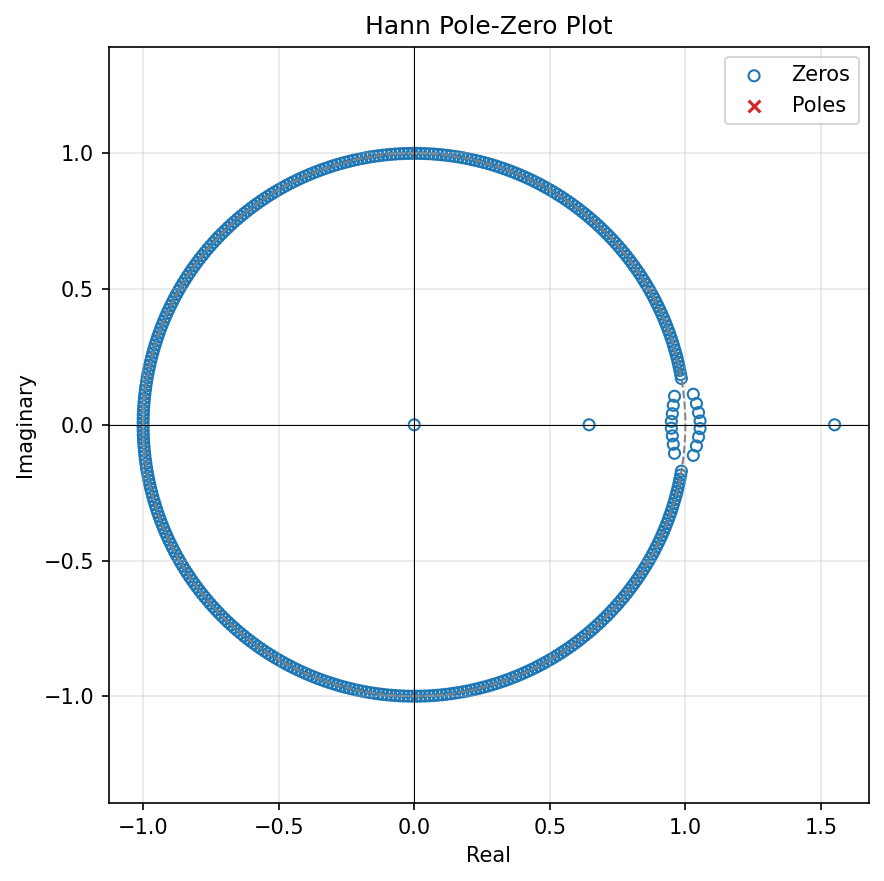
\includegraphics[width=\textwidth]{lab02_fig02_hann_pz.png}
    \caption{Pole-zero plot}
    \label{fig:hann_pz}
  \end{subfigure}
  \hfill
  \begin{subfigure}{0.48\textwidth}
    \centering
    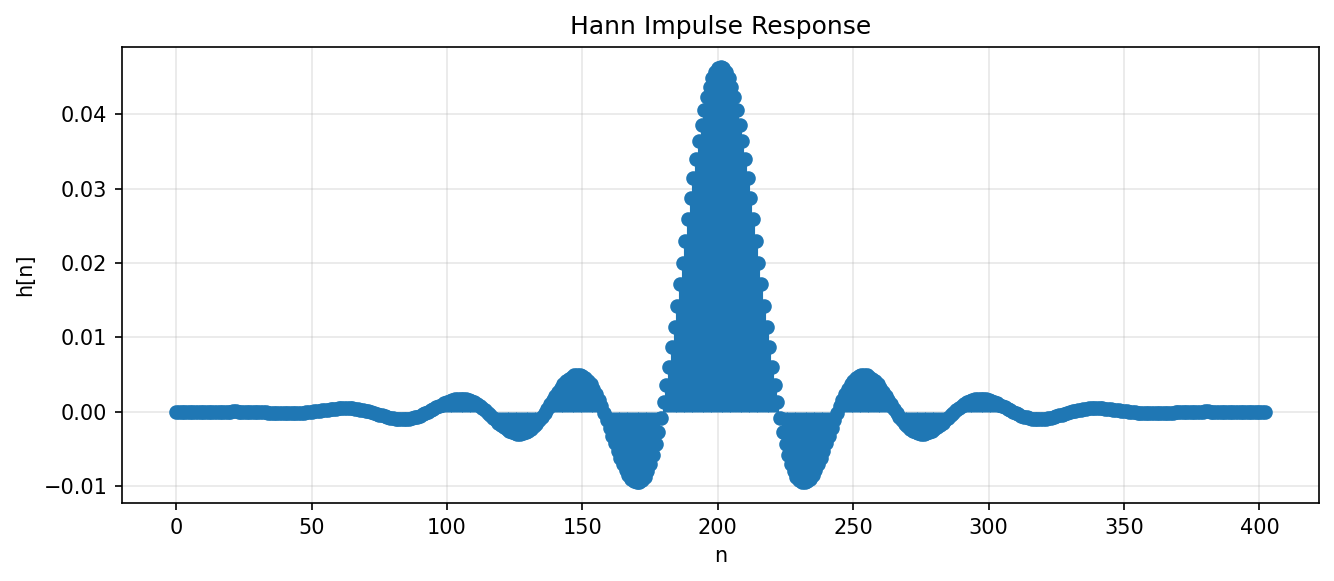
\includegraphics[width=\textwidth]{lab02_fig03_hann_impulse.png}
    \caption{Impulse response}
    \label{fig:hann_imp}
  \end{subfigure}
  \caption{Hann FIR pole-zero plot and impulse response.}
\end{figure}

\begin{figure}[H]
  \centering
  \begin{subfigure}{0.32\textwidth}
    \centering
    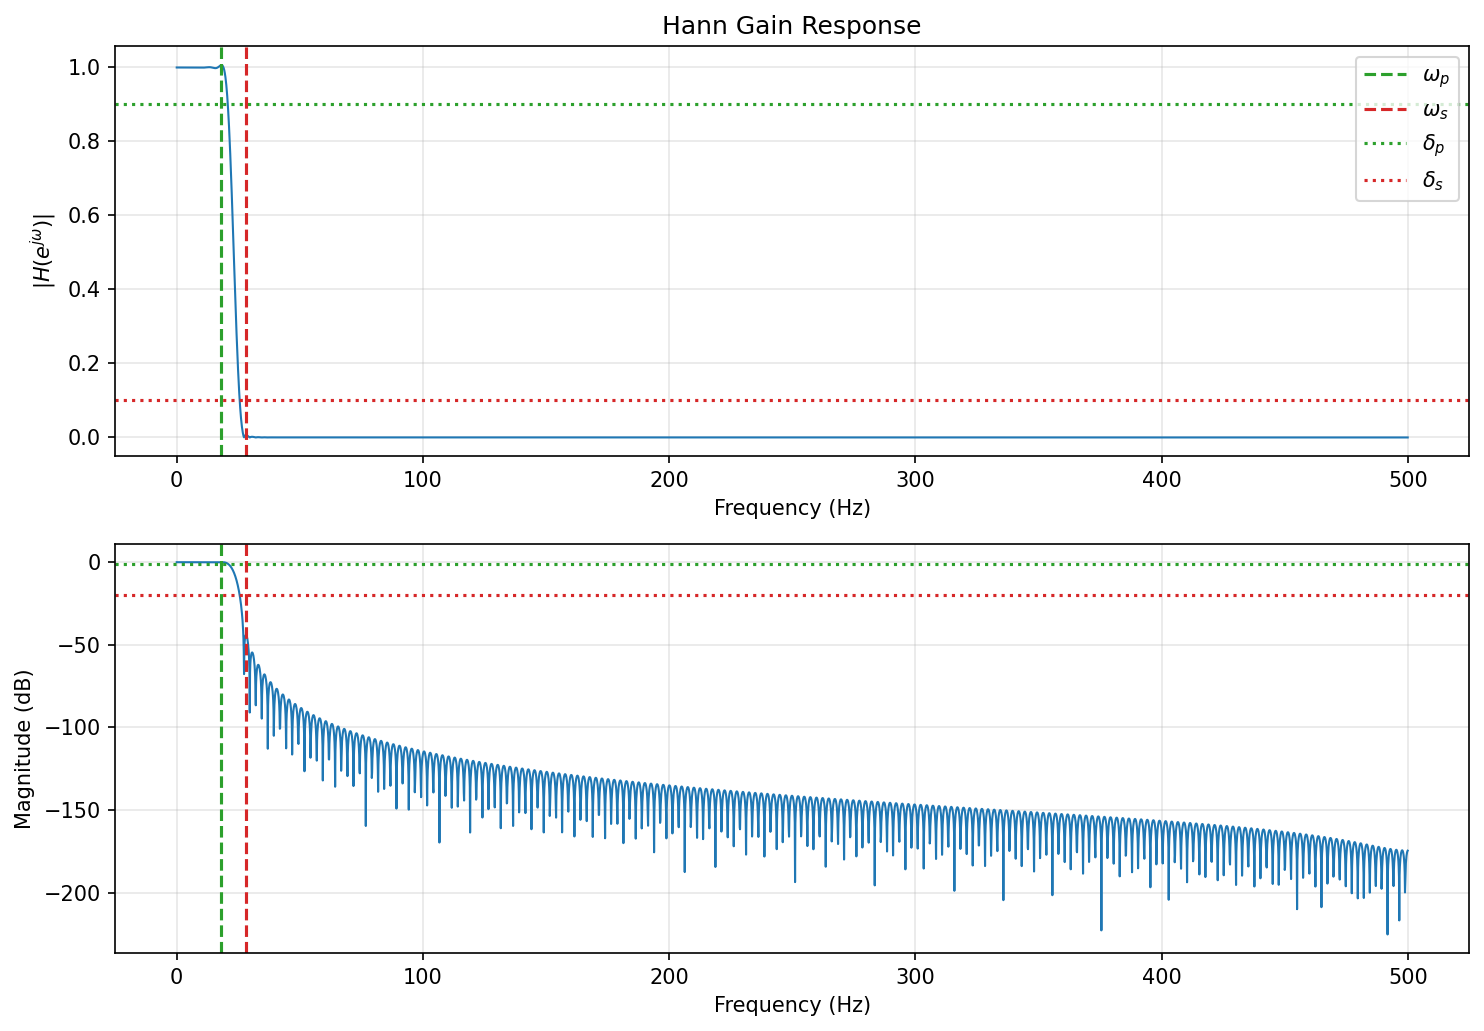
\includegraphics[width=\textwidth]{lab02_fig04_hann_gain.png}
    \caption{Gain response}
    \label{fig:hann_gain}
  \end{subfigure}
  \hfill
  \begin{subfigure}{0.32\textwidth}
    \centering
    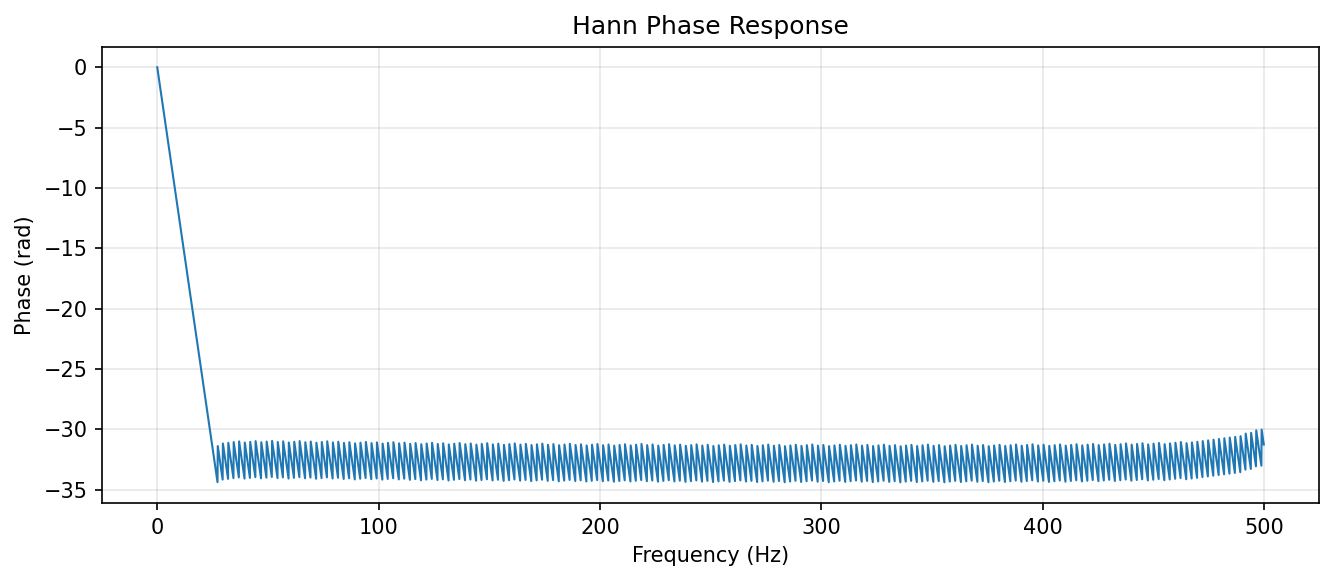
\includegraphics[width=\textwidth]{lab02_fig05_hann_phase.png}
    \caption{Phase response}
    \label{fig:hann_phase}
  \end{subfigure}
  \hfill
  \begin{subfigure}{0.32\textwidth}
    \centering
    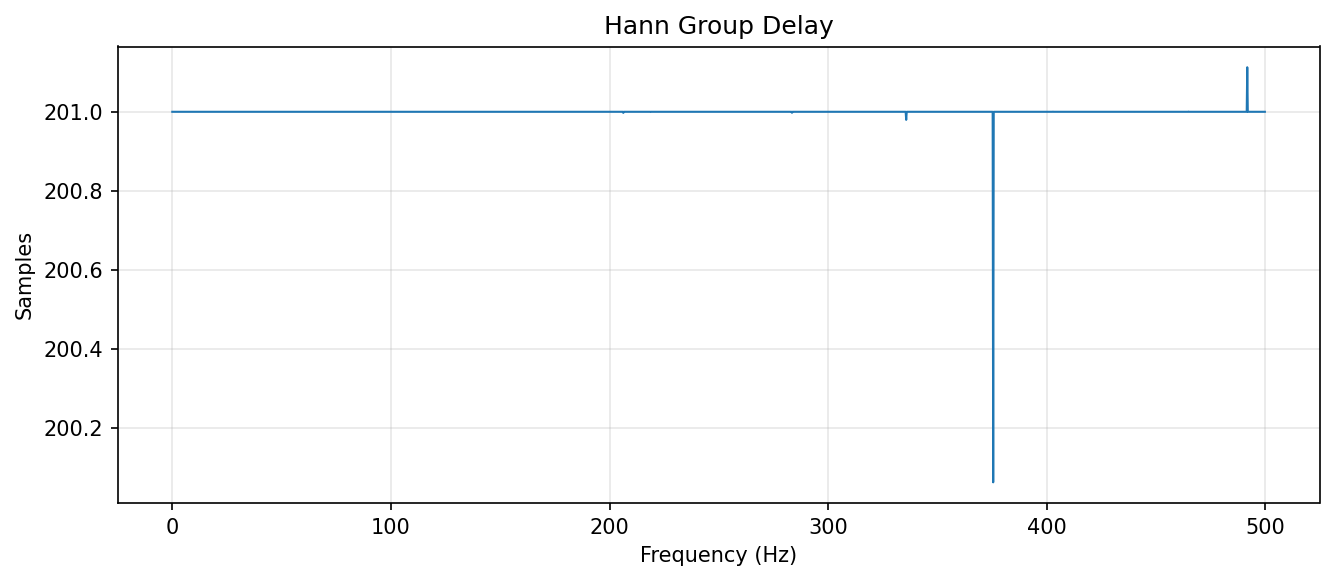
\includegraphics[width=\textwidth]{lab02_fig06_hann_gd.png}
    \caption{Group delay}
    \label{fig:hann_gd}
  \end{subfigure}
  \caption{Hann FIR gain, phase, and group-delay characteristics.}
\end{figure}

The smooth window taper reduces sidelobe energy significantly, so the gain response is smoother and more selective. The constant group delay confirms the expected linear-phase behavior.

\subsection{Hamming Window FIR}
Figures~\ref{fig:hamming_pz}--\ref{fig:hamming_gd} summarize the Hamming window design. The verified response gives $\min |H| = 0.9980$ and $\max |H| = 0.00173$, so the stopband is cleaner than the Hann case while preserving the same overall order.
\begin{figure}[H]
  \centering
  \begin{subfigure}{0.48\textwidth}
    \centering
    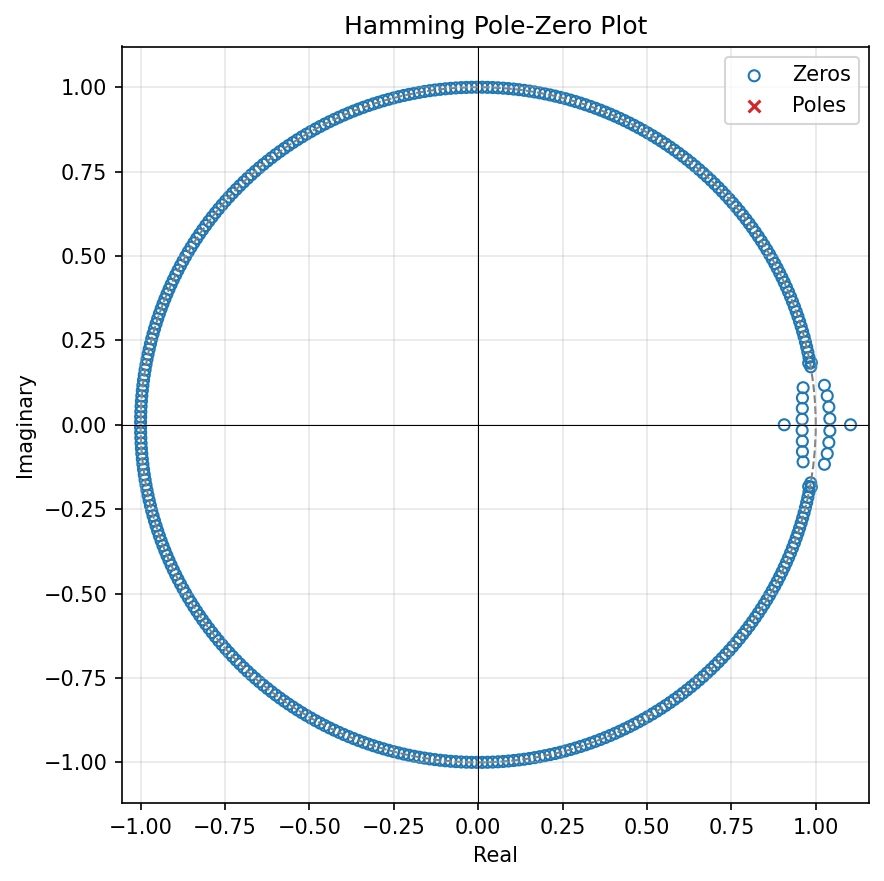
\includegraphics[width=\textwidth]{lab02_fig02_hamming_pz.png}
    \caption{Pole-zero plot}
    \label{fig:hamming_pz}
  \end{subfigure}
  \hfill
  \begin{subfigure}{0.48\textwidth}
    \centering
    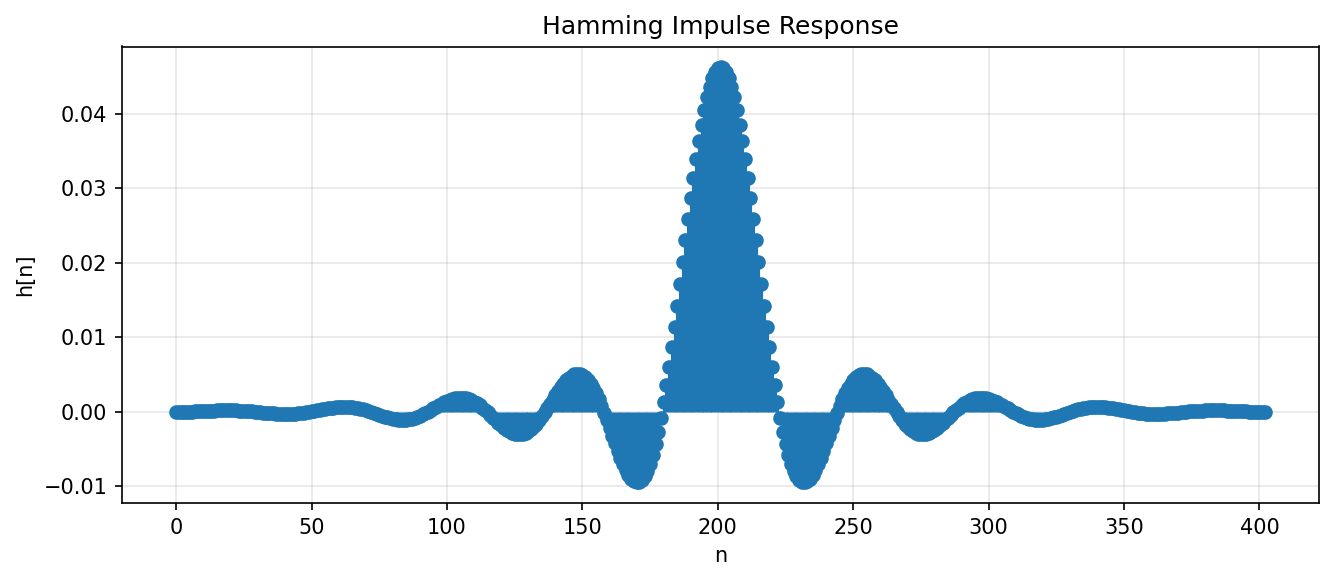
\includegraphics[width=\textwidth]{lab02_fig03_hamming_impulse.png}
    \caption{Impulse response}
    \label{fig:hamming_imp}
  \end{subfigure}
  \caption{Hamming FIR pole-zero plot and impulse response.}
\end{figure}

\begin{figure}[H]
  \centering
  \begin{subfigure}{0.32\textwidth}
    \centering
    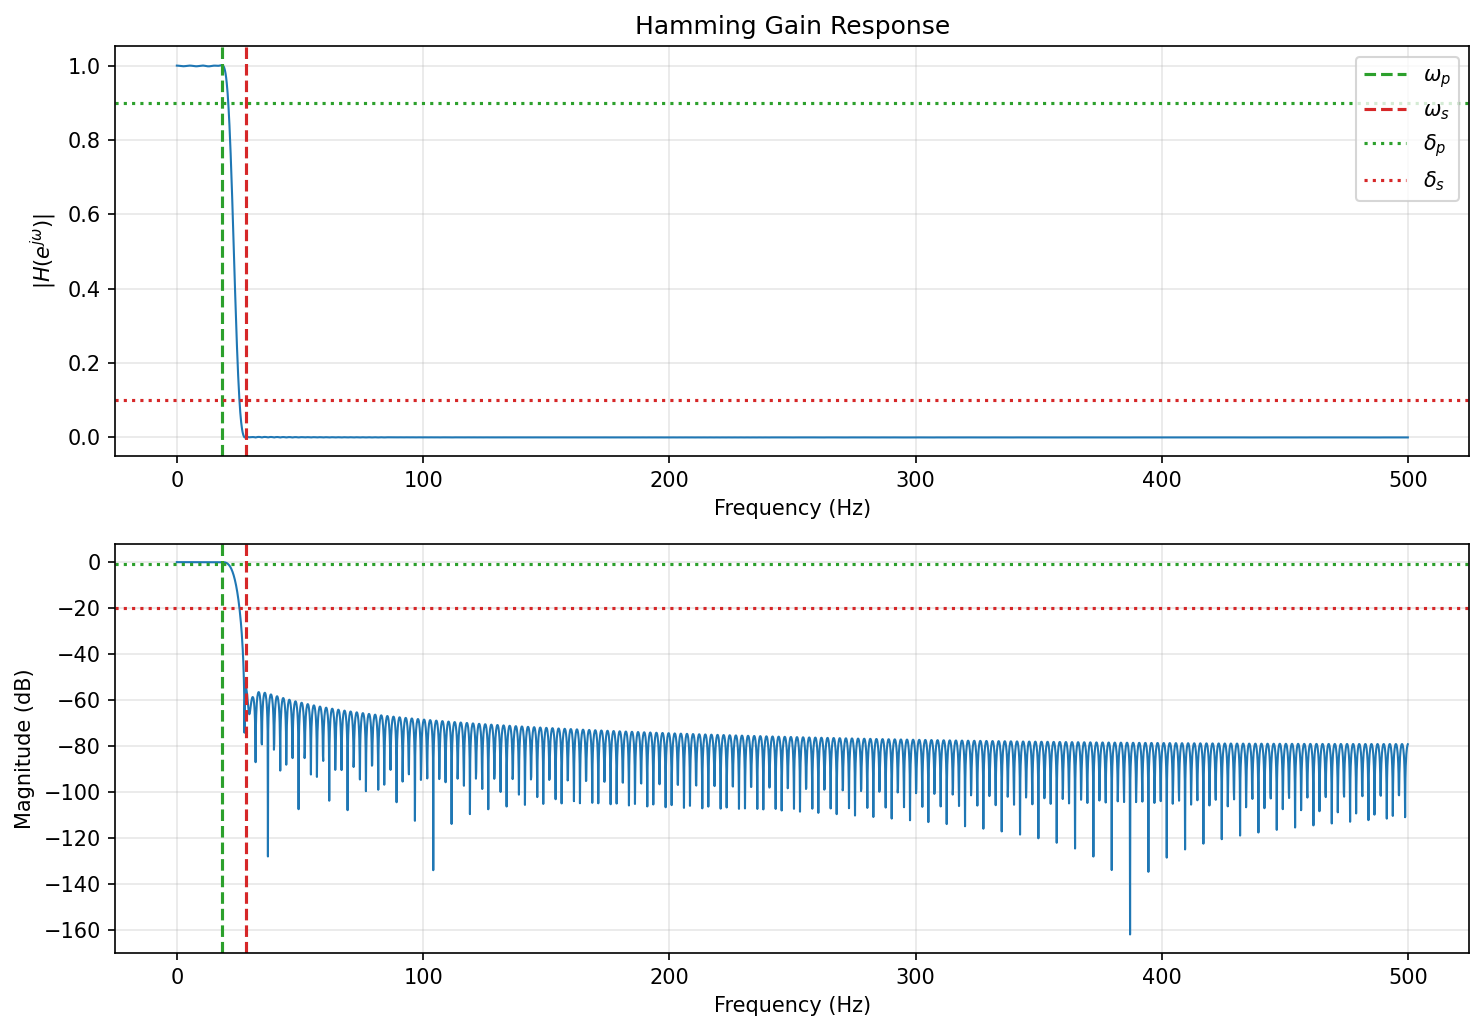
\includegraphics[width=\textwidth]{lab02_fig04_hamming_gain.png}
    \caption{Gain response}
    \label{fig:hamming_gain}
  \end{subfigure}
  \hfill
  \begin{subfigure}{0.32\textwidth}
    \centering
    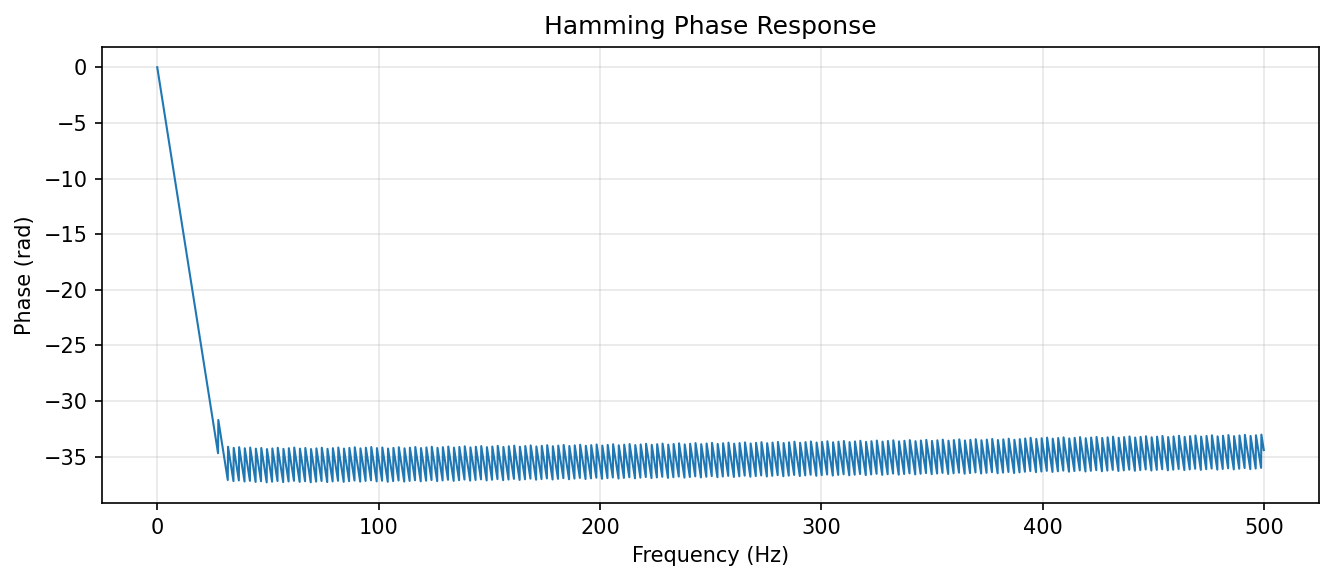
\includegraphics[width=\textwidth]{lab02_fig05_hamming_phase.png}
    \caption{Phase response}
    \label{fig:hamming_phase}
  \end{subfigure}
  \hfill
  \begin{subfigure}{0.32\textwidth}
    \centering
    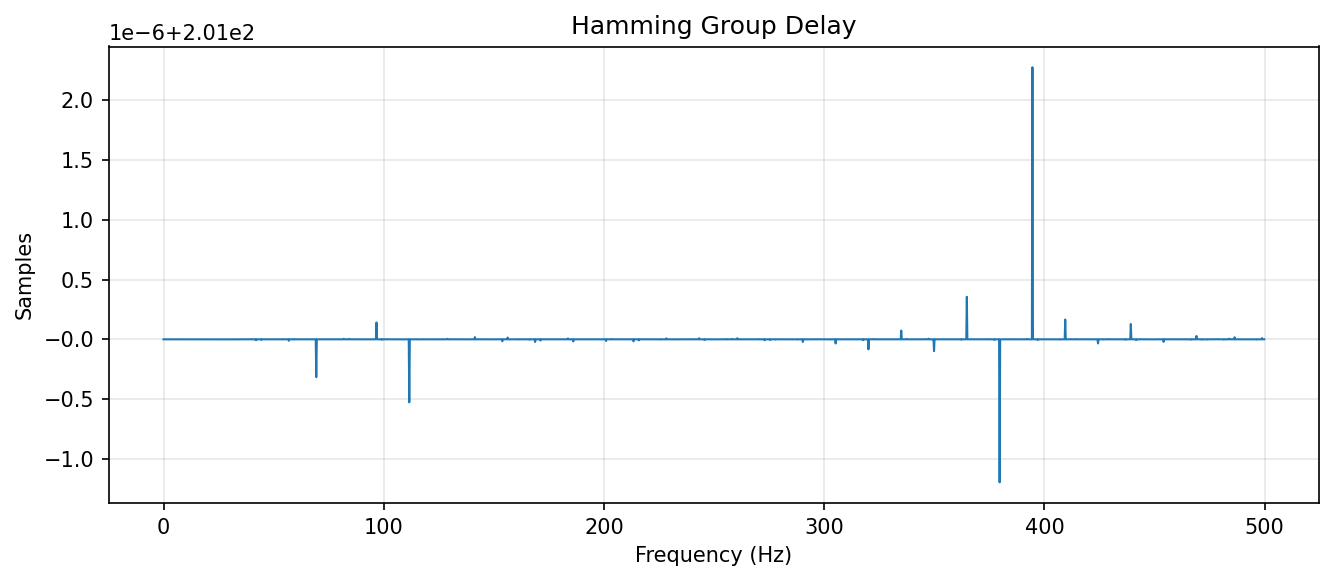
\includegraphics[width=\textwidth]{lab02_fig06_hamming_gd.png}
    \caption{Group delay}
    \label{fig:hamming_gd}
  \end{subfigure}
  \caption{Hamming FIR gain, phase, and group-delay characteristics.}
\end{figure}

The Hamming response confirms why this window is often a practical default in FIR work: it keeps very low sidelobe levels while remaining straightforward to design and implement.

\subsection{Blackman Window FIR}
Figures~\ref{fig:black_pz}--\ref{fig:black_gd} show the Blackman window design. The response is extremely clean, with $\min |H| = 0.9999$ and $\max |H| = 1.71 \times 10^{-4}$, but the order rises to 602.
\begin{figure}[H]
  \centering
  \begin{subfigure}{0.48\textwidth}
    \centering
    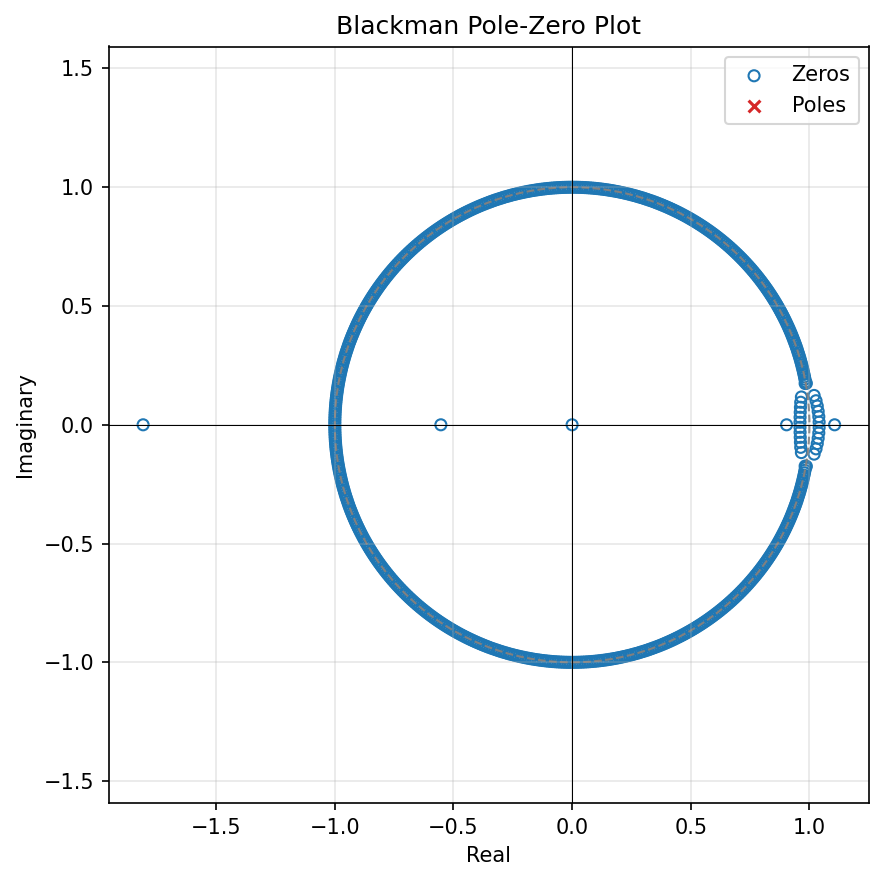
\includegraphics[width=\textwidth]{lab02_fig02_blackman_pz.png}
    \caption{Pole-zero plot}
    \label{fig:black_pz}
  \end{subfigure}
  \hfill
  \begin{subfigure}{0.48\textwidth}
    \centering
    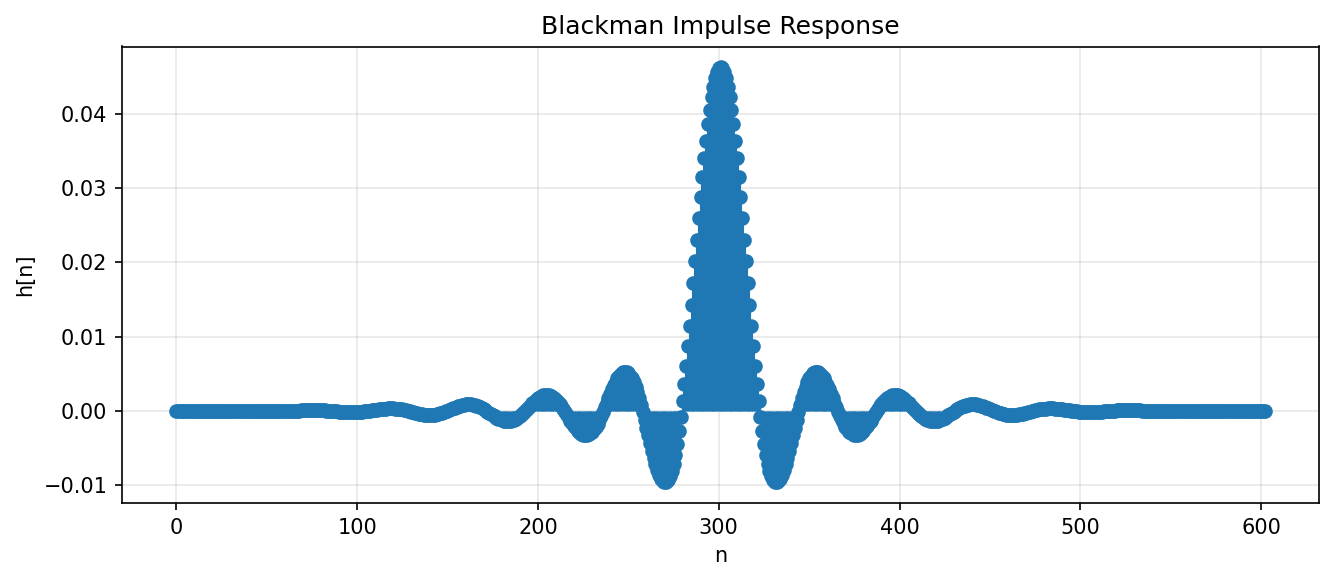
\includegraphics[width=\textwidth]{lab02_fig03_blackman_impulse.png}
    \caption{Impulse response}
    \label{fig:black_imp}
  \end{subfigure}
  \caption{Blackman FIR pole-zero plot and impulse response.}
\end{figure}

\begin{figure}[H]
  \centering
  \begin{subfigure}{0.32\textwidth}
    \centering
    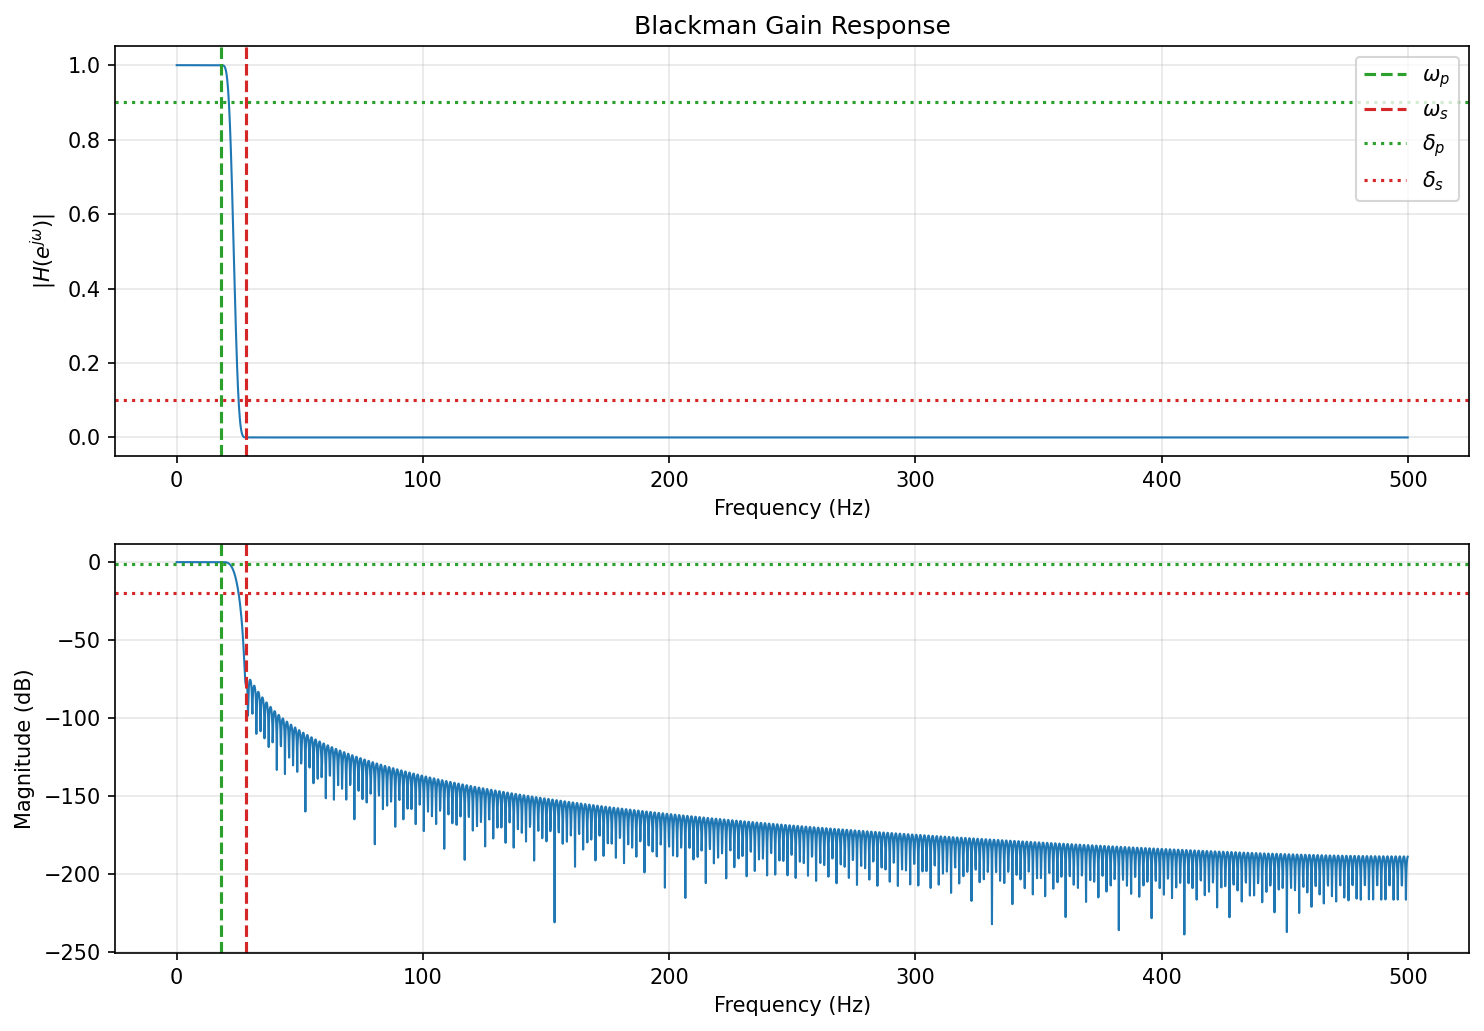
\includegraphics[width=\textwidth]{lab02_fig04_blackman_gain.png}
    \caption{Gain response}
    \label{fig:black_gain}
  \end{subfigure}
  \hfill
  \begin{subfigure}{0.32\textwidth}
    \centering
    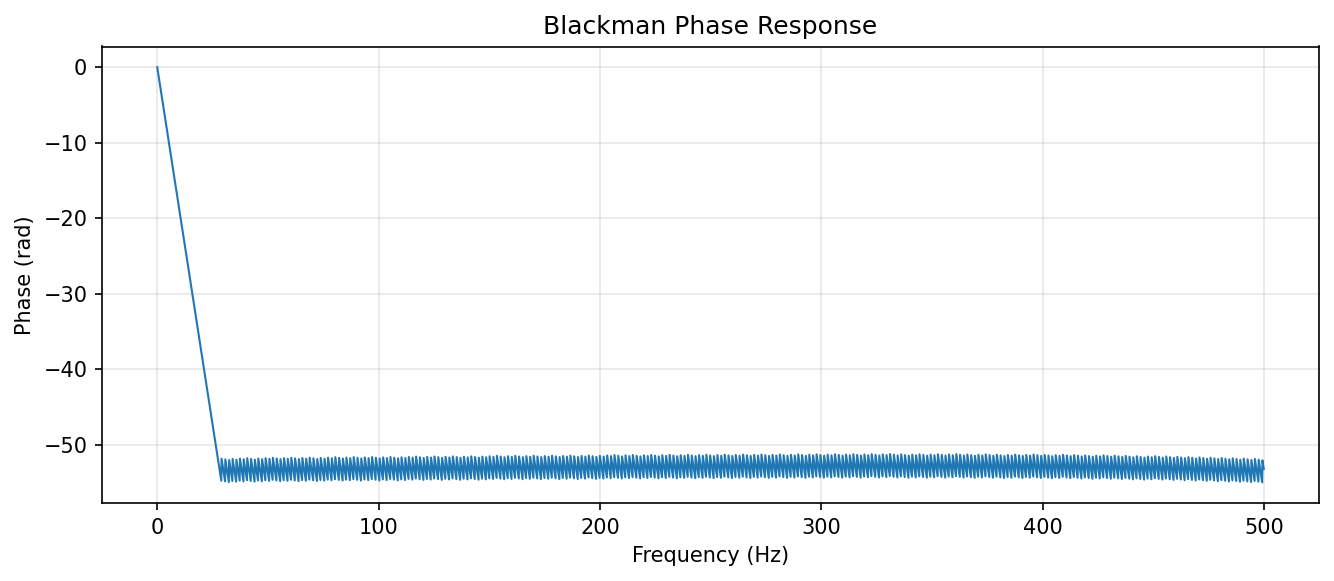
\includegraphics[width=\textwidth]{lab02_fig05_blackman_phase.png}
    \caption{Phase response}
    \label{fig:black_phase}
  \end{subfigure}
  \hfill
  \begin{subfigure}{0.32\textwidth}
    \centering
    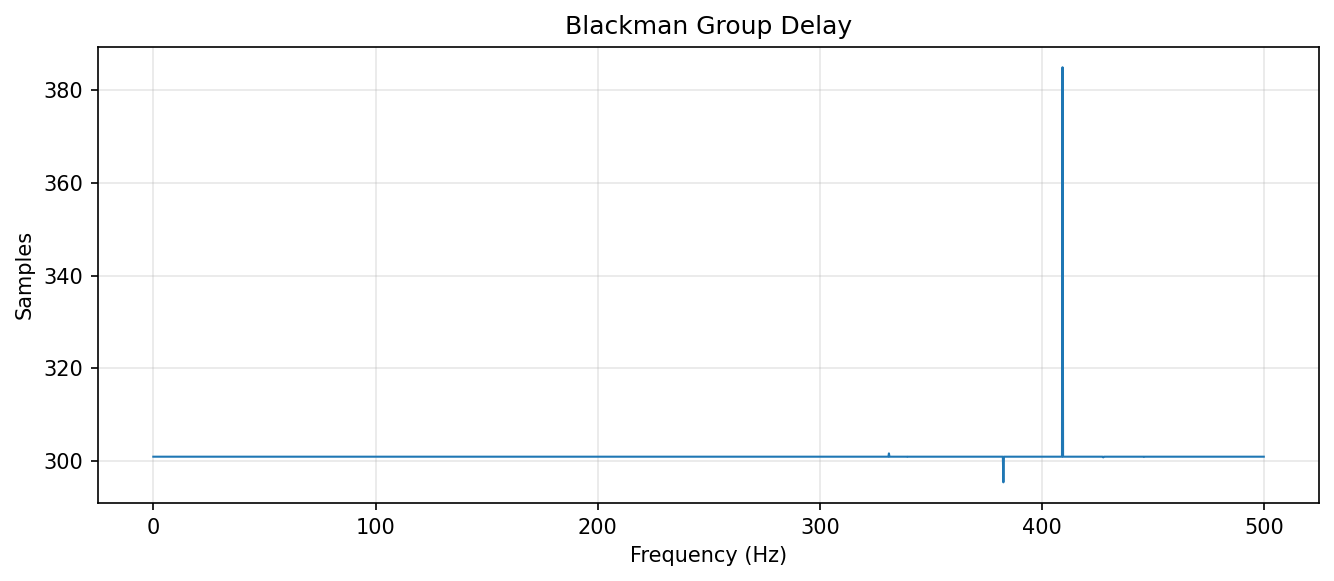
\includegraphics[width=\textwidth]{lab02_fig06_blackman_gd.png}
    \caption{Group delay}
    \label{fig:black_gd}
  \end{subfigure}
  \caption{Blackman FIR gain, phase, and group-delay characteristics.}
\end{figure}

This filter provides the best stopband rejection among the window-method designs in this laboratory, but it also has the largest convolution cost because of its long impulse response.

\section{Task 4: White Gaussian Noise Input Analysis}
Task 4 required each filter to process a unit-power white Gaussian noise input of length 1000. The filtered outputs are shown in Figs.~\ref{fig:noise_butter}--\ref{fig:noise_blackman}.

Figure~\ref{fig:noise_butter} shows the Butterworth output. The time-domain waveform remains noise-like, but the DFT magnitude and the autocorrelation-based power spectrum clearly suppress energy above the stopband edge.
\begin{figure}[H]
  \centering
  
\includegraphics[width=0.86\textwidth]{lab02_noise_butter.png}
  \caption{Butterworth response to white Gaussian noise.}
  \label{fig:noise_butter}
\end{figure}

Figure~\ref{fig:noise_cheby1} shows the Chebyshev Type I output. The passband ripple produces slightly more uneven in-band shaping than the Butterworth design, but the transition is sharper because the filter order is lower.
\begin{figure}[H]
  \centering
  
\includegraphics[width=0.86\textwidth]{lab02_noise_cheby1.png}
  \caption{Chebyshev Type I response to white Gaussian noise.}
  \label{fig:noise_cheby1}
\end{figure}

Figure~\ref{fig:noise_cheby2} shows the Chebyshev Type II output. The stopband rejection is strong and the spectral floor above the cutoff is clearly reduced.
\begin{figure}[H]
  \centering
  
\includegraphics[width=0.86\textwidth]{lab02_noise_cheby2.png}
  \caption{Chebyshev Type II response to white Gaussian noise.}
  \label{fig:noise_cheby2}
\end{figure}

Figure~\ref{fig:noise_box} shows the boxcar FIR output. The noise is visibly bandlimited, but the stopband leakage remains larger than in the smoother FIR windows.
\begin{figure}[H]
  \centering
  
\includegraphics[width=0.86\textwidth]{lab02_noise_boxcar.png}
  \caption{Boxcar FIR response to white Gaussian noise.}
  \label{fig:noise_box}
\end{figure}

Figure~\ref{fig:noise_bart} shows the Bartlett FIR output, where the power spectrum becomes cleaner above the cutoff than in the boxcar case because of improved sidelobe suppression.
\begin{figure}[H]
  \centering
  
\includegraphics[width=0.86\textwidth]{lab02_noise_bartlett.png}
  \caption{Bartlett FIR response to white Gaussian noise.}
  \label{fig:noise_bart}
\end{figure}

Figure~\ref{fig:noise_hann} shows the Hann FIR output. The remaining stopband energy is much smaller than for the rectangular and triangular windows.
\begin{figure}[H]
  \centering
  
\includegraphics[width=0.86\textwidth]{lab02_noise_hann.png}
  \caption{Hann FIR response to white Gaussian noise.}
  \label{fig:noise_hann}
\end{figure}

Figure~\ref{fig:noise_hamming} shows the Hamming FIR output, which further reduces stopband leakage and keeps a very smooth in-band response.
\begin{figure}[H]
  \centering
  
\includegraphics[width=0.86\textwidth]{lab02_noise_hamming.png}
  \caption{Hamming FIR response to white Gaussian noise.}
  \label{fig:noise_hamming}
\end{figure}

Figure~\ref{fig:noise_blackman} shows the Blackman FIR output. Its power spectrum has the cleanest stopband of the FIR set, which matches the response-metric table from the verified code.
\begin{figure}[H]
  \centering
  
\includegraphics[width=0.86\textwidth]{lab02_noise_blackman.png}
  \caption{Blackman FIR response to white Gaussian noise.}
  \label{fig:noise_blackman}
\end{figure}

Overall, all eight filters concentrate output power below the passband edge. The IIR filters achieve that concentration with very low order, but their phase is nonlinear. The FIR filters require long impulse responses, yet they preserve linear phase and show progressively better stopband cleanliness from boxcar to Blackman \cite{oppenheim2010, proakis2007, harris1978}.

\section{Task 5: Chirp Signal Input Analysis}
The chirp input is
\begin{equation}
x(t) = \sin\left(2\pi \frac{t^2}{100}\right), \qquad 0 \le t \le 100,\qquad F_s = 1000\ \text{Sa/s}.
\end{equation}
Its instantaneous frequency is
\begin{equation}
f_i(t) = \frac{d}{dt}\left(\frac{t^2}{100}\right) = \frac{t}{50}\ \text{Hz},
\end{equation}
so the chirp sweeps only from 0 Hz to 2 Hz over the full duration. Since this is far below the passband edge of 18.1786 Hz, the filters are expected to pass the chirp almost entirely, with the main differences arising from passband flatness and phase behavior.

The Butterworth response in Fig.~\ref{fig:chirp_butter} confirms this expectation: the chirp remains visible across the full record, and the spectrogram shows essentially complete transmission in the low-frequency region.
\begin{figure}[H]
  \centering
  
\includegraphics[width=0.86\textwidth]{lab02_chirp_butter.png}
  \caption{Butterworth response to the chirp input.}
  \label{fig:chirp_butter}
\end{figure}

The Chebyshev Type I response in Fig.~\ref{fig:chirp_cheby1} also passes the chirp fully, though the passband ripple causes slightly different amplitude shaping than the Butterworth case.
\begin{figure}[H]
  \centering
  
\includegraphics[width=0.86\textwidth]{lab02_chirp_cheby1.png}
  \caption{Chebyshev Type I response to the chirp input.}
  \label{fig:chirp_cheby1}
\end{figure}

The Chebyshev Type II response in Fig.~\ref{fig:chirp_cheby2} similarly preserves the chirp because the entire sweep lies well inside the passband.
\begin{figure}[H]
  \centering
  
\includegraphics[width=0.86\textwidth]{lab02_chirp_cheby2.png}
  \caption{Chebyshev Type II response to the chirp input.}
  \label{fig:chirp_cheby2}
\end{figure}

The boxcar FIR output in Fig.~\ref{fig:chirp_box} passes the chirp, but the long FIR delay is evident in the time-domain trace.
\begin{figure}[H]
  \centering
  
\includegraphics[width=0.86\textwidth]{lab02_chirp_boxcar.png}
  \caption{Boxcar FIR response to the chirp input.}
  \label{fig:chirp_box}
\end{figure}

The Bartlett FIR result in Fig.~\ref{fig:chirp_bart} again shows nearly complete transmission of the chirp energy, with the spectrogram remaining concentrated below a few hertz.
\begin{figure}[H]
  \centering
  
\includegraphics[width=0.86\textwidth]{lab02_chirp_bartlett.png}
  \caption{Bartlett FIR response to the chirp input.}
  \label{fig:chirp_bart}
\end{figure}

The Hann FIR response in Fig.~\ref{fig:chirp_hann} confirms the same low-frequency transmission, now with extremely clean out-of-band suppression.
\begin{figure}[H]
  \centering
  
\includegraphics[width=0.86\textwidth]{lab02_chirp_hann.png}
  \caption{Hann FIR response to the chirp input.}
  \label{fig:chirp_hann}
\end{figure}

The Hamming FIR response in Fig.~\ref{fig:chirp_hamming} is similarly transparent to the chirp because the entire sweep remains inside the passband.
\begin{figure}[H]
  \centering
  
\includegraphics[width=0.86\textwidth]{lab02_chirp_hamming.png}
  \caption{Hamming FIR response to the chirp input.}
  \label{fig:chirp_hamming}
\end{figure}

The Blackman FIR response in Fig.~\ref{fig:chirp_blackman} also preserves the chirp almost perfectly while maintaining the cleanest rejection of any hypothetical higher-frequency content.
\begin{figure}[H]
  \centering
  
\includegraphics[width=0.86\textwidth]{lab02_chirp_blackman.png}
  \caption{Blackman FIR response to the chirp input.}
  \label{fig:chirp_blackman}
\end{figure}

Because the chirp never enters the transition or stopband, this task mainly highlights passband behavior rather than cutoff behavior. All eight filters transmit the chirp, but the IIR filters do so with nonlinear phase and short memory, whereas the FIR filters do so with long, linear-phase delay.

\section{Conclusion}
This laboratory compared IIR and FIR low-pass filters under a common set of design specifications derived from E/21/291. The IIR filters required orders 7, 4, and 4 for Butterworth, Chebyshev Type I, and Chebyshev Type II, respectively, showing the expected efficiency advantage of recursive designs. The FIR window methods required much higher orders, ranging from 200 for the boxcar filter to 602 for the Blackman filter, because linear phase and direct window control are obtained at the expense of impulse-response length.

Among the IIR filters, the Butterworth response was maximally flat but needed the highest IIR order. The Chebyshev Type I filter achieved the same specification at lower order by allowing passband ripple, while the Chebyshev Type II filter placed the ripple in the stopband instead. Among the FIR filters, the boxcar design had the poorest sidelobe behavior, the Bartlett filter improved the stopband, the Hann and Hamming windows produced strong all-around performance, and the Blackman window delivered the best stopband rejection at the highest order \cite{oppenheim2010, proakis2007, mitra2011, antoniou2018, parks1987, harris1978, rabiner1975}.

In practical applications, IIR filters are attractive when low order and computational efficiency are dominant requirements, especially in embedded or real-time systems. FIR filters are preferred when linear phase is important, such as in data communications, biomedical waveform preservation, and multirate processing. The results of this laboratory therefore illustrate the real engineering trade-off between recursive efficiency and phase-controlled fidelity.

\begin{thebibliography}{99}
\bibitem{oppenheim2010}
A. V. Oppenheim and R. W. Schafer, \textit{Discrete-Time Signal Processing}, 3rd ed. Upper Saddle River, NJ, USA: Prentice-Hall, 2010.

\bibitem{proakis2007}
J. G. Proakis and D. G. Manolakis, \textit{Digital Signal Processing: Principles, Algorithms, and Applications}, 4th ed. Upper Saddle River, NJ, USA: Prentice-Hall, 2007.

\bibitem{mitra2011}
S. K. Mitra, \textit{Digital Signal Processing: A Computer-Based Approach}, 4th ed. New York, NY, USA: McGraw-Hill, 2011.

\bibitem{antoniou2018}
A. Antoniou, \textit{Digital Filters: Analysis, Design, and Signal Processing Applications}, 2nd ed. New York, NY, USA: McGraw-Hill, 2018.

\bibitem{parks1987}
T. W. Parks and C. S. Burrus, \textit{Digital Filter Design}. New York, NY, USA: Wiley-Interscience, 1987.

\bibitem{oppenheim1997}
A. V. Oppenheim, A. S. Willsky, and S. H. Nawab, \textit{Signals and Systems}, 2nd ed. Upper Saddle River, NJ, USA: Prentice-Hall, 1997.

\bibitem{harris1978}
F. J. Harris, ``On the use of windows for harmonic analysis with the discrete Fourier transform,'' \textit{Proc. IEEE}, vol. 66, no. 1, pp. 51--83, Jan. 1978.

\bibitem{rabiner1975}
L. R. Rabiner and B. Gold, \textit{Theory and Application of Digital Signal Processing}. Englewood Cliffs, NJ, USA: Prentice-Hall, 1975.
\end{thebibliography}

\appendix
\section{Python Source Code}

\subsection{Filter Parameter Computation}
\begin{lstlisting}[caption={Imports, helper functions, and parameter computation for Lab 02.}, label={lst:lab02_params}]
import json
import math
from pathlib import Path

import matplotlib
matplotlib.use("Agg")
import matplotlib.pyplot as plt
import numpy as np
from scipy import signal


OUTPUT_DIR = Path(".")


def save_figure(filename: str) -> None:
    plt.savefig(OUTPUT_DIR / filename, dpi=150, bbox_inches="tight")
    plt.close("all")


def impulse_response(b: np.ndarray, a: np.ndarray, length: int) -> np.ndarray:
    impulse = np.zeros(length)
    impulse[0] = 1.0
    return signal.lfilter(b, a, impulse)


def noise_power_spectrum(y: np.ndarray, fs: float) -> tuple[np.ndarray, np.ndarray]:
    corr = signal.correlate(y, y, mode="full", method="fft")
    power = np.abs(np.fft.fft(np.fft.ifftshift(corr)))
    freqs = np.fft.fftfreq(len(corr), d=1.0 / fs)
    mask = freqs >= 0.0
    return freqs[mask], power[mask]


def response_metrics(freqs_hz: np.ndarray, magnitude: np.ndarray, fp_hz: float, fs_hz: float) -> dict:
    passband_mask = freqs_hz <= fp_hz
    stopband_mask = freqs_hz >= fs_hz
    return {
        "min_passband_gain": float(np.min(magnitude[passband_mask])),
        "max_stopband_gain": float(np.max(magnitude[stopband_mask])),
    }


def iir_transfer_summary(sos: np.ndarray) -> list[list[float]]:
    return [[float(value) for value in row] for row in sos]


def main() -> None:
    a, b, c, d = 2, 9, 1, 3
    fs = 1000.0
    delta_s = 0.1
    delta_p = 0.9
    delta_t = 0.1

    wp = 100.0 + math.sqrt(1.1 * a + 11.0 * b + 101.0 * c)
    ws = wp * (1.0 + math.sqrt(d / 10.0))
    fp_hz = wp / (2.0 * math.pi)
    fs_hz = ws / (2.0 * math.pi)
    wc = 0.5 * (wp + ws)
    fc_hz = wc / (2.0 * math.pi)

    omega_p = 2.0 * fs * math.tan(wp / (2.0 * fs))
    omega_s = 2.0 * fs * math.tan(ws / (2.0 * fs))
    epsilon_p = math.sqrt(1.0 / (delta_p**2) - 1.0)
    epsilon_s = math.sqrt(1.0 / (delta_s**2) - 1.0)
    omega_ratio = omega_s / omega_p

    butter_order_manual = math.ceil(math.log(epsilon_s / epsilon_p) / math.log(omega_ratio))
    cheby_order_manual = math.ceil(math.acosh(epsilon_s / epsilon_p) / math.acosh(omega_ratio))

    rp_db = -20.0 * math.log10(delta_p)
    rs_db = -20.0 * math.log10(delta_s)
    butter_order_scipy, butter_wn = signal.buttord(omega_p, omega_s, rp_db, rs_db, analog=True)
    cheby1_order_scipy, cheby1_wn = signal.cheb1ord(omega_p, omega_s, rp_db, rs_db, analog=True)
    cheby2_order_scipy, cheby2_wn = signal.cheb2ord(omega_p, omega_s, rp_db, rs_db, analog=True)

    delta_omega_normalized = (ws - wp) / fs
    fir_orders = {
        "boxcar": math.ceil(4.0 * math.pi / delta_omega_normalized) - 1,
        "bartlett": math.ceil(8.0 * math.pi / delta_omega_normalized) - 1,
        "hann": math.ceil(8.0 * math.pi / delta_omega_normalized) - 1,
        "hamming": math.ceil(8.0 * math.pi / delta_omega_normalized) - 1,
        "blackman": math.ceil(12.0 * math.pi / delta_omega_normalized) - 1,
    }
    for key, order in list(fir_orders.items()):
        if order % 2 != 0:
            fir_orders[key] = order + 1
\end{lstlisting}

\subsection{IIR Filter Design: Butterworth}
\begin{lstlisting}[caption={Butterworth analog prototype design and bilinear-transform conversion.}, label={lst:lab02_butter}]
    butter_ba_analog = signal.butter(butter_order_scipy, butter_wn, btype="low", analog=True, output="ba")
    butter_bz = signal.bilinear(*butter_ba_analog, fs=fs)

    filters = {
        "butter": {
            "display": "Butterworth",
            "kind": "IIR",
            "b": np.asarray(butter_bz[0], dtype=float),
            "a": np.asarray(butter_bz[1], dtype=float),
            "sos": signal.tf2sos(*butter_bz),
            "order": int(butter_order_scipy),
        },
    }
\end{lstlisting}

\subsection{IIR Filter Design: Chebyshev Type I}
\begin{lstlisting}[caption={Chebyshev Type I design code.}, label={lst:lab02_cheby1}]
    cheby1_ba_analog = signal.cheby1(
        cheby1_order_scipy, rp_db, cheby1_wn, btype="low", analog=True, output="ba"
    )
    cheby1_bz = signal.bilinear(*cheby1_ba_analog, fs=fs)

    filters["cheby1"] = {
        "display": "Chebyshev Type I",
        "kind": "IIR",
        "b": np.asarray(cheby1_bz[0], dtype=float),
        "a": np.asarray(cheby1_bz[1], dtype=float),
        "sos": signal.tf2sos(*cheby1_bz),
        "order": int(cheby1_order_scipy),
    }
\end{lstlisting}

\subsection{IIR Filter Design: Chebyshev Type II}
\begin{lstlisting}[caption={Chebyshev Type II design code.}, label={lst:lab02_cheby2}]
    cheby2_ba_analog = signal.cheby2(
        cheby2_order_scipy, rs_db, cheby2_wn, btype="low", analog=True, output="ba"
    )
    cheby2_bz = signal.bilinear(*cheby2_ba_analog, fs=fs)

    filters["cheby2"] = {
        "display": "Chebyshev Type II",
        "kind": "IIR",
        "b": np.asarray(cheby2_bz[0], dtype=float),
        "a": np.asarray(cheby2_bz[1], dtype=float),
        "sos": signal.tf2sos(*cheby2_bz),
        "order": int(cheby2_order_scipy),
    }
\end{lstlisting}

\subsection{FIR Filter Design: Window Methods}
\begin{lstlisting}[caption={FIR window-method designs for Lab 02.}, label={lst:lab02_fir}]
    for name, order in fir_orders.items():
        numtaps = order + 1
        filters[name] = {
            "display": name.capitalize() if name != "boxcar" else "Boxcar",
            "kind": "FIR",
            "b": signal.firwin(numtaps, fc_hz, window=name, fs=fs),
            "a": np.array([1.0]),
            "sos": [],
            "order": int(order),
        }

    noise_input = np.random.default_rng(291).standard_normal(1000)
    t_noise = np.arange(noise_input.size) / fs
    t_chirp = np.linspace(0.0, 100.0, int(100.0 * fs) + 1)
    chirp_input = np.sin(2.0 * np.pi * t_chirp**2 / 100.0)
\end{lstlisting}

\subsection{Frequency Response and Pole-Zero Plotting}
\begin{lstlisting}[caption={Loop that generates pole-zero, impulse, gain, phase, and group-delay figures.}, label={lst:lab02_plots}]
    results = {
        "student": {"e_number": "E/21/291", "a": a, "b": b, "c": c, "d": d},
        "specifications": {
            "wp_rad_per_s": wp,
            "ws_rad_per_s": ws,
            "fp_hz": fp_hz,
            "fs_hz": fs_hz,
            "wc_rad_per_s": wc,
            "fc_hz": fc_hz,
            "omega_p_prewarped": omega_p,
            "omega_s_prewarped": omega_s,
            "epsilon_p": epsilon_p,
            "epsilon_s": epsilon_s,
            "omega_ratio": omega_ratio,
            "delta_omega_normalized": delta_omega_normalized,
            "delta_t": delta_t,
        },
        "orders": {
            "manual": {
                "butterworth": butter_order_manual,
                "chebyshev_type_i": cheby_order_manual,
                "chebyshev_type_ii": cheby_order_manual,
                "boxcar": fir_orders["boxcar"],
                "bartlett": fir_orders["bartlett"],
                "hann": fir_orders["hann"],
                "hamming": fir_orders["hamming"],
                "blackman": fir_orders["blackman"],
            },
            "scipy": {
                "butterworth": int(butter_order_scipy),
                "chebyshev_type_i": int(cheby1_order_scipy),
                "chebyshev_type_ii": int(cheby2_order_scipy),
            },
        },
        "filters": {},
    }

    short_name_to_display = {
        "butter": "Butterworth",
        "cheby1": "Chebyshev Type I",
        "cheby2": "Chebyshev Type II",
        "boxcar": "Boxcar",
        "bartlett": "Bartlett",
        "hann": "Hann",
        "hamming": "Hamming",
        "blackman": "Blackman",
    }

    for short_name, config in filters.items():
        b_coeff = np.asarray(config["b"], dtype=float)
        a_coeff = np.asarray(config["a"], dtype=float)

        z, p, _ = signal.tf2zpk(b_coeff, a_coeff)
        freq_axis, response = signal.freqz(b_coeff, a_coeff, worN=4096, fs=fs)
        magnitude = np.abs(response)
        magnitude_db = 20.0 * np.log10(magnitude + 1e-12)
        phase = np.unwrap(np.angle(response))
        gd_freqs, gd_values = signal.group_delay((b_coeff, a_coeff), w=2048, fs=fs)
        metrics = response_metrics(freq_axis, magnitude, fp_hz, fs_hz)

        plt.figure(figsize=(6, 6))
        plt.scatter(np.real(z), np.imag(z), s=28, facecolors="none", edgecolors="tab:blue", label="Zeros")
        plt.scatter(np.real(p), np.imag(p), s=32, marker="x", color="tab:red", label="Poles")
        circle = plt.Circle((0.0, 0.0), 1.0, fill=False, linestyle="--", color="gray")
        plt.gca().add_patch(circle)
        plt.axhline(0.0, color="black", linewidth=0.5)
        plt.axvline(0.0, color="black", linewidth=0.5)
        plt.title(f"{short_name_to_display[short_name]} Pole-Zero Plot")
        plt.xlabel("Real")
        plt.ylabel("Imaginary")
        plt.axis("equal")
        plt.grid(True, alpha=0.3)
        plt.legend(loc="upper right")
        plt.tight_layout()
        save_figure(f"lab02_fig02_{short_name}_pz.png")

        impulse_len = 220 if config["kind"] == "IIR" else len(b_coeff)
        h = impulse_response(b_coeff, a_coeff, impulse_len)
        plt.figure(figsize=(9, 4))
        plt.stem(np.arange(impulse_len), h, basefmt=" ")
        plt.title(f"{short_name_to_display[short_name]} Impulse Response")
        plt.xlabel("n")
        plt.ylabel("h[n]")
        plt.grid(True, alpha=0.3)
        plt.tight_layout()
        save_figure(f"lab02_fig03_{short_name}_impulse.png")

        plt.figure(figsize=(10, 7))
        plt.subplot(2, 1, 1)
        plt.plot(freq_axis, magnitude, linewidth=1.0)
        plt.axvline(fp_hz, color="tab:green", linestyle="--", label=r"$\omega_p$")
        plt.axvline(fs_hz, color="tab:red", linestyle="--", label=r"$\omega_s$")
        plt.axhline(delta_p, color="tab:green", linestyle=":", label=r"$\delta_p$")
        plt.axhline(delta_s, color="tab:red", linestyle=":", label=r"$\delta_s$")
        plt.title(f"{short_name_to_display[short_name]} Gain Response")
        plt.xlabel("Frequency (Hz)")
        plt.ylabel(r"$|H(e^{j\omega})|$")
        plt.grid(True, alpha=0.3)
        plt.legend(loc="upper right")
        plt.subplot(2, 1, 2)
        plt.plot(freq_axis, magnitude_db, linewidth=1.0)
        plt.axvline(fp_hz, color="tab:green", linestyle="--")
        plt.axvline(fs_hz, color="tab:red", linestyle="--")
        plt.axhline(20.0 * math.log10(delta_p), color="tab:green", linestyle=":")
        plt.axhline(20.0 * math.log10(delta_s), color="tab:red", linestyle=":")
        plt.xlabel("Frequency (Hz)")
        plt.ylabel("Magnitude (dB)")
        plt.grid(True, alpha=0.3)
        plt.tight_layout()
        save_figure(f"lab02_fig04_{short_name}_gain.png")

        plt.figure(figsize=(9, 4))
        plt.plot(freq_axis, phase, linewidth=1.0)
        plt.title(f"{short_name_to_display[short_name]} Phase Response")
        plt.xlabel("Frequency (Hz)")
        plt.ylabel("Phase (rad)")
        plt.grid(True, alpha=0.3)
        plt.tight_layout()
        save_figure(f"lab02_fig05_{short_name}_phase.png")

        plt.figure(figsize=(9, 4))
        plt.plot(gd_freqs, gd_values, linewidth=1.0)
        plt.title(f"{short_name_to_display[short_name]} Group Delay")
        plt.xlabel("Frequency (Hz)")
        plt.ylabel("Samples")
        plt.grid(True, alpha=0.3)
        plt.tight_layout()
        save_figure(f"lab02_fig06_{short_name}_gd.png")
\end{lstlisting}

\subsection{White Gaussian Noise Analysis}
\begin{lstlisting}[caption={Noise-input analysis for all eight Lab 02 filters.}, label={lst:lab02_noise}]
        noise_output = signal.lfilter(b_coeff, a_coeff, noise_input)
        noise_fft = np.fft.fft(noise_output)
        noise_freqs = np.fft.fftfreq(noise_output.size, d=1.0 / fs)
        noise_mask = noise_freqs >= 0.0
        psd_freqs, psd_values = noise_power_spectrum(noise_output, fs)

        plt.figure(figsize=(10, 8))
        plt.subplot(3, 1, 1)
        plt.plot(t_noise, noise_output, linewidth=0.8)
        plt.title(f"{short_name_to_display[short_name]} Output for White Gaussian Noise")
        plt.xlabel("Time (s)")
        plt.ylabel("Amplitude")
        plt.grid(True, alpha=0.3)
        plt.subplot(3, 1, 2)
        plt.plot(noise_freqs[noise_mask], np.abs(noise_fft[noise_mask]), linewidth=0.8)
        plt.title("One-Sided DFT Magnitude")
        plt.xlabel("Frequency (Hz)")
        plt.ylabel(r"$|Y[k]|$")
        plt.grid(True, alpha=0.3)
        plt.subplot(3, 1, 3)
        plt.plot(psd_freqs, psd_values, linewidth=0.8)
        plt.title("Power Spectrum from the FFT of the Autocorrelation")
        plt.xlabel("Frequency (Hz)")
        plt.ylabel("Power")
        plt.grid(True, alpha=0.3)
        plt.tight_layout()
        save_figure(f"lab02_noise_{short_name}.png")
\end{lstlisting}

\subsection{Chirp Signal Analysis}
\begin{lstlisting}[caption={Chirp-input analysis, results export, and script termination for Lab 02.}, label={lst:lab02_chirp}]
        chirp_output = signal.lfilter(b_coeff, a_coeff, chirp_input)
        chirp_spec_f, chirp_spec_t, chirp_spec = signal.spectrogram(
            chirp_output, fs=fs, nperseg=4096, noverlap=3072, scaling="density"
        )

        plt.figure(figsize=(10, 8))
        plt.subplot(2, 1, 1)
        plt.plot(t_chirp, chirp_output, linewidth=0.7)
        plt.title(f"{short_name_to_display[short_name]} Output for the Chirp Input")
        plt.xlabel("Time (s)")
        plt.ylabel("Amplitude")
        plt.grid(True, alpha=0.3)
        plt.subplot(2, 1, 2)
        plt.pcolormesh(
            chirp_spec_t,
            chirp_spec_f,
            10.0 * np.log10(chirp_spec + 1e-12),
            shading="auto",
        )
        plt.ylim(0.0, 30.0)
        plt.title("Output Spectrogram")
        plt.xlabel("Time (s)")
        plt.ylabel("Frequency (Hz)")
        plt.colorbar(label="Power/Frequency (dB/Hz)")
        plt.tight_layout()
        save_figure(f"lab02_chirp_{short_name}.png")

        results["filters"][short_name] = {
            "display_name": short_name_to_display[short_name],
            "type": config["kind"],
            "order": config["order"],
            "num_degree": len(b_coeff) - 1,
            "den_degree": len(a_coeff) - 1,
            "numerator": [float(value) for value in b_coeff],
            "denominator": [float(value) for value in a_coeff],
            "sos": iir_transfer_summary(config["sos"]) if config["kind"] == "IIR" else [],
            "min_passband_gain": metrics["min_passband_gain"],
            "max_stopband_gain": metrics["max_stopband_gain"],
            "max_pole_radius": float(np.max(np.abs(p))) if p.size else 0.0,
        }

    with open(OUTPUT_DIR / "lab02_results.json", "w", encoding="utf-8") as file:
        json.dump(results, file, indent=2)

    print(json.dumps(results, indent=2))


if __name__ == "__main__":
    main()
\end{lstlisting}

\end{document}
